\documentclass{cskkuproject}

% ==========================================
% ข้อมูลโครงงาน — กรอกข้อมูลที่นี่
% ==========================================

\titleTH{Pacegasus: ระบบผู้ช่วยออกแบบ จัดตาราง และปรับแผนการวิ่งเฉพาะบุคคล}
\titleEN{Pacegasus: Personal Running Plan \& Schedule Assistant}

% ข้อมูลนักศึกษาคนที่ 1
\firstStudentID{663380225-9}
\firstStudentPrefixTH{นาย}
\firstStudentNameTH{พีรัชชัย สืบสิงห์}
\firstStudentNameEN{Pheeratchai Suepsing}

% ข้อมูลนักศึกษาคนที่ 2
% *** ถ้าทำโครงงานคนเดียว ให้เว้นว่างไว้ทั้งหมด (เหมือนด้านล่าง) ***
% *** ถ้ามี 2 คน ให้กรอกข้อมูลเหมือนคนที่ 1 ***
\secondStudentID{663380514-2}
\secondStudentPrefixTH{นาย}
\secondStudentNameTH{เบญจพล บุบผามาลา}
\secondStudentNameEN{Banchpol Bubphamala}

% ข้อมูลหลักสูตร
\degreeTH{วิทยาศาสตรบัณฑิต}
\degreeEN{Bachelor of Science}
\majorTH{วิทยาการคอมพิวเตอร์}
\majorEN{Computer Science}

% อาจารย์ที่ปรึกษา
\advisorTH{ผศ. ดร. ชิตสุธา สุ่มเล็ก}
\advisorEN{Asst. Prof. Chitsutha Soomlek, Ph.D.}

% ปีการศึกษา
\academicYearTH{2569}
\academicYearEN{2026}

% รหัสวิชา (CP354 771 = โครงงาน 1, CP354 772 = โครงงาน 2)
\courseCode{CP354 771}
\courseName{โครงงานคอมพิวเตอร์ 1}
\semester{1}

% คำสำคัญ
\keywordsTH{แอปพลิเคชันวิ่ง, เกมมิฟิเคชัน, การปรับแผนฝึกอัตโนมัติ, แรงจูงใจในการออกกำลังกาย, ระบบสังคมออนไลน์}
\keywordsEN{Running Application, Gamification, Adaptive Training, Exercise Motivation, Social Interaction}


\begin{document}

% ==========================================
% หน้าปก
% ==========================================
% คำสั่งด้านล่างสร้างหน้าปกอัตโนมัติจากข้อมูลที่กรอกด้านบน
% ไม่ต้องแก้ไขส่วนนี้
\makeprogresscover{1}

% ตั้งค่าเลขหน้าส่วนต้นเป็นอักษรไทย (ก, ข, ค, ...)
\pagenumbering{arabic}
\setcounter{page}{0}
\renewcommand{\thepage}{\ThaiAlph{\value{page}}}

% ==========================================
% บทคัดย่อ
% ==========================================
\begin{abstractTH}
% บทคัดย่อภาษาไทย
% หมายเหตุ: ไม่ควรเกิน 300 คำ
% ควรครอบคลุม: วัตถุประสงค์ → วิธีการ → ผลลัพธ์ → การประยุกต์ใช้
%
โครงงานนี้มีวัตถุประสงค์เพื่อออกแบบและพัฒนาแอปพลิเคชันบนมือถือชื่อ ``Pacegasus'' สำหรับส่งเสริมพฤติกรรมการวิ่งออกกำลังกายอย่างยั่งยืน โดยผสานแนวคิดเกมมิฟิเคชัน (Gamification) เข้ากับการปรับแผนฝึกอัตโนมัติและระบบปฏิสัมพันธ์ทางสังคม บนพื้นฐานทฤษฎีการกำหนดใจตนเอง (Self-Determination Theory: SDT) และเทคนิคการเปลี่ยนพฤติกรรม (Behavior Change Techniques: BCTs)

ระบบพัฒนาบนแพลตฟอร์ม React Native รองรับระบบปฏิบัติการ Android โดยใช้เซนเซอร์ GPS และ Accelerometer ในตัวสมาร์ตโฟนเพื่อติดตามระยะทาง ความเร็วเฉลี่ย (Pace) และจำนวนก้าว โดยไม่จำเป็นต้องพึ่งพาอุปกรณ์เสริมภายนอก ฝั่งเซิร์ฟเวอร์ใช้ Node.js และ PostgreSQL สำหรับประมวลผลและจัดเก็บข้อมูล

ฟีเจอร์หลักของระบบประกอบด้วยเอนจินปรับแผนฝึกอัตโนมัติ (Adaptive Training Engine) ที่วิเคราะห์ข้อมูลสุขภาวะรายวัน ค่า Session-RPE และอัตราส่วนภาระฝึกระยะเฉียบพลันต่อเรื้อรัง (ACWR) เพื่อปรับมิชชั่นรายวันและรายสัปดาห์ให้เหมาะสมกับแต่ละบุคคล ระบบเกมมิฟิเคชันที่ประกอบด้วยคะแนน เหรียญตรา กระดานจัดอันดับ และโหมดเนื้อเรื่อง ตลอดจนระบบสังคมที่เปิดให้ผู้ใช้เพิ่มเพื่อน เข้าร่วมกิจกรรมกลุ่ม และแชร์ผลการวิ่ง

ผลที่คาดว่าจะได้รับจากโครงงานนี้คือต้นแบบแอปพลิเคชันที่ใช้งานได้จริง ซึ่งสามารถช่วยเพิ่มความสม่ำเสมอในการออกกำลังกาย ลดความเสี่ยงจากการบาดเจ็บ และส่งเสริมพฤติกรรมสุขภาพที่ยั่งยืนในระยะยาว อันเป็นแนวทางหนึ่งในการบรรเทาปัญหาโรคไม่ติดต่อเรื้อรัง (NCDs) ในระดับประชากร

\end{abstractTH}

\begin{abstractEN}
% ABSTRACT (English)
% Note: Should not exceed 300 words.
% Should cover: Objective, Methodology, Results, Applications
% Use Past tense for objectives and methodology
% Use Present tense for results and applications
%
This project aims to design and develop a mobile application named ``Pacegasus'' to promote sustainable running behavior. The system integrates Gamification principles with an Adaptive Training Engine and a social interaction framework, grounded in Self-Determination Theory (SDT) and Behavior Change Techniques (BCTs).

The application is developed using React Native for cross-platform Android deployment, leveraging built-in smartphone sensors---GPS and Accelerometer---to track distance, average pace, and step count without requiring external wearable devices. The backend is powered by Node.js and PostgreSQL for data processing and storage.

Key features include an Adaptive Training Engine that analyzes daily wellness check-in data, Session-RPE scores, and the Acute-to-Chronic Workload Ratio (ACWR) to personalize daily and weekly missions. Gamification elements such as points, badges, leaderboards, and a Story Mode are incorporated alongside social features enabling users to add friends, join group activities, and share running results.

The expected outcome is a functional prototype capable of improving exercise adherence, reducing injury risk, and fostering long-term healthy behaviors---contributing to the mitigation of Non-Communicable Diseases (NCDs) at the population level.

\end{abstractEN}

% ==========================================
% กิตติกรรมประกาศ
% ==========================================
\begin{acknowledgement}
โครงงานคอมพิวเตอร์ฉบับนี้สำเร็จลุล่วงได้ด้วยดี เนื่องจากได้รับความกรุณาและการสนับสนุนจากบุคคลหลายท่าน ที่คณะผู้จัดทำขอกราบขอบพระคุณเป็นอย่างยิ่ง

ขอกราบขอบพระคุณ ผู้ช่วยศาสตราจารย์ ดร. ชิตสุธา สุ่มเล็ก อาจารย์ที่ปรึกษาโครงงาน สาขาวิชาวิทยาการคอมพิวเตอร์ วิทยาลัยการคอมพิวเตอร์ มหาวิทยาลัยขอนแก่น ที่ได้กรุณาให้คำปรึกษา แนะนำแนวทาง และตรวจสอบโครงงานนี้อย่างละเอียด ทั้งในด้านวิชาการและการดำเนินงาน ด้วยความเอาใจใส่และอุทิศเวลาตลอดมา ความรู้ ประสบการณ์ และคำแนะนำอันมีค่าของท่านเป็นแรงผลักดันสำคัญที่ทำให้งานชิ้นนี้บรรลุผลสำเร็จ

สุดท้ายนี้ ขอกราบขอบพระคุณบิดามารดาและครอบครัวทุกท่าน ที่ให้การสนับสนุน ให้กำลังใจ และเป็นแรงบันดาลใจที่ยิ่งใหญ่ตลอดมา คุณค่าและความสำเร็จของโครงงานนี้ ขอมอบเป็นกตัญญุตาแด่บิดามารดาและผู้มีพระคุณทุกท่าน

\begin{flushright}
ผู้จัดทำ\\
นายพีรัชชัย สืบสิงห์\\
นายเบญจพล บุบผามาลา
\end{flushright}

\end{acknowledgement}

% ==========================================
% สารบัญ
% ==========================================
\tableofcontents
\clearpage
\listoffigures
\clearpage
\listoftables
\clearpage

% ==========================================
% สัญลักษณ์และคำย่อ (ถ้ามี — uncomment ด้านล่าง)
% ==========================================
% \begin{symbolpage}
% \input{symbols}
% \end{symbolpage}

% ==========================================
% เนื้อเรื่อง 5 บท
% ==========================================
% เริ่มนับเลขหน้าใหม่เป็นเลขอารบิก (1, 2, 3, ...)
% ไม่ต้องแก้ไขส่วนนี้
\pagenumbering{arabic}
\setcounter{page}{1}

\chapterone
\chaptertwo
\chapterthree
\chapterfour
\chapterfive

% ==========================================
% เอกสารอ้างอิง
% ==========================================
% *** ไม่ต้องแก้ไขส่วนนี้ ***
% ระบบจะดึงรายการอ้างอิงจากไฟล์ references.bib อัตโนมัติ
% ให้แก้ไขรายการอ้างอิงในไฟล์ references.bib แทน
\clearpage
\addcontentsline{toc}{chapter}{เอกสารอ้างอิง}
\makeatletter
\let\ps@plain\ps@empty
\makeatother
\bibliographystyle{ieeetr}
\bibliography{references}

% ==========================================
% ภาคผนวก
% ==========================================
% เพิ่มไฟล์ appendices.tex และเปิดบรรทัดนี้เมื่อมีภาคผนวก
% % =============================
% ภาคผนวก
% =============================
% หมายเหตุ: ก่อนเริ่มภาคผนวก ระบบจะสร้างหน้าคั่นให้อัตโนมัติ
% ใช้คำสั่ง \appendiceschapter{ชื่อภาคผนวก} สำหรับแต่ละภาคผนวก
% ระบบจะกำหนดตัวอักษร ก, ข, ค ... ให้โดยอัตโนมัติ
%
% *** ลบข้อความตัวอย่างด้านล่าง แล้วใส่ภาพ UI / Prototype ของตนเอง ***

% =============================
% ภาคผนวก ก
% =============================
\setcounter{chapter}{-1}
\appendiceschapter{ตัวอย่าง UI หรือ Prototype}

\section*{ผลการพัฒนาแอปพลิเคชัน}

ภาคผนวกนี้แสดงภาพหน้าจอของแอปพลิเคชันต้นแบบ Pacegasus ซึ่งพัฒนาขึ้นตามลำดับการใช้งานจริง ตั้งแต่การเข้าสู่ระบบ การกรอกข้อมูล การเลือกแผนการฝึก การวิ่ง และการรับรางวัล

\subsection*{การเข้าสู่ระบบและการสมัครสมาชิก}

หน้าจอเข้าสู่ระบบรองรับการกรอกอีเมลและการเข้าสู่ระบบด้วย Google ส่วนหน้าจอสมัครสมาชิกช่วยให้ผู้ใช้สร้างบัญชีใหม่ รวมถึงหน้าข้อกำหนดและการยินยอม และหน้าสำหรับยืนยันตัวตนด้วยรหัส OTP

\begin{figure}[H]\centering
\begin{subfigure}[t]{0.31\textwidth}\centering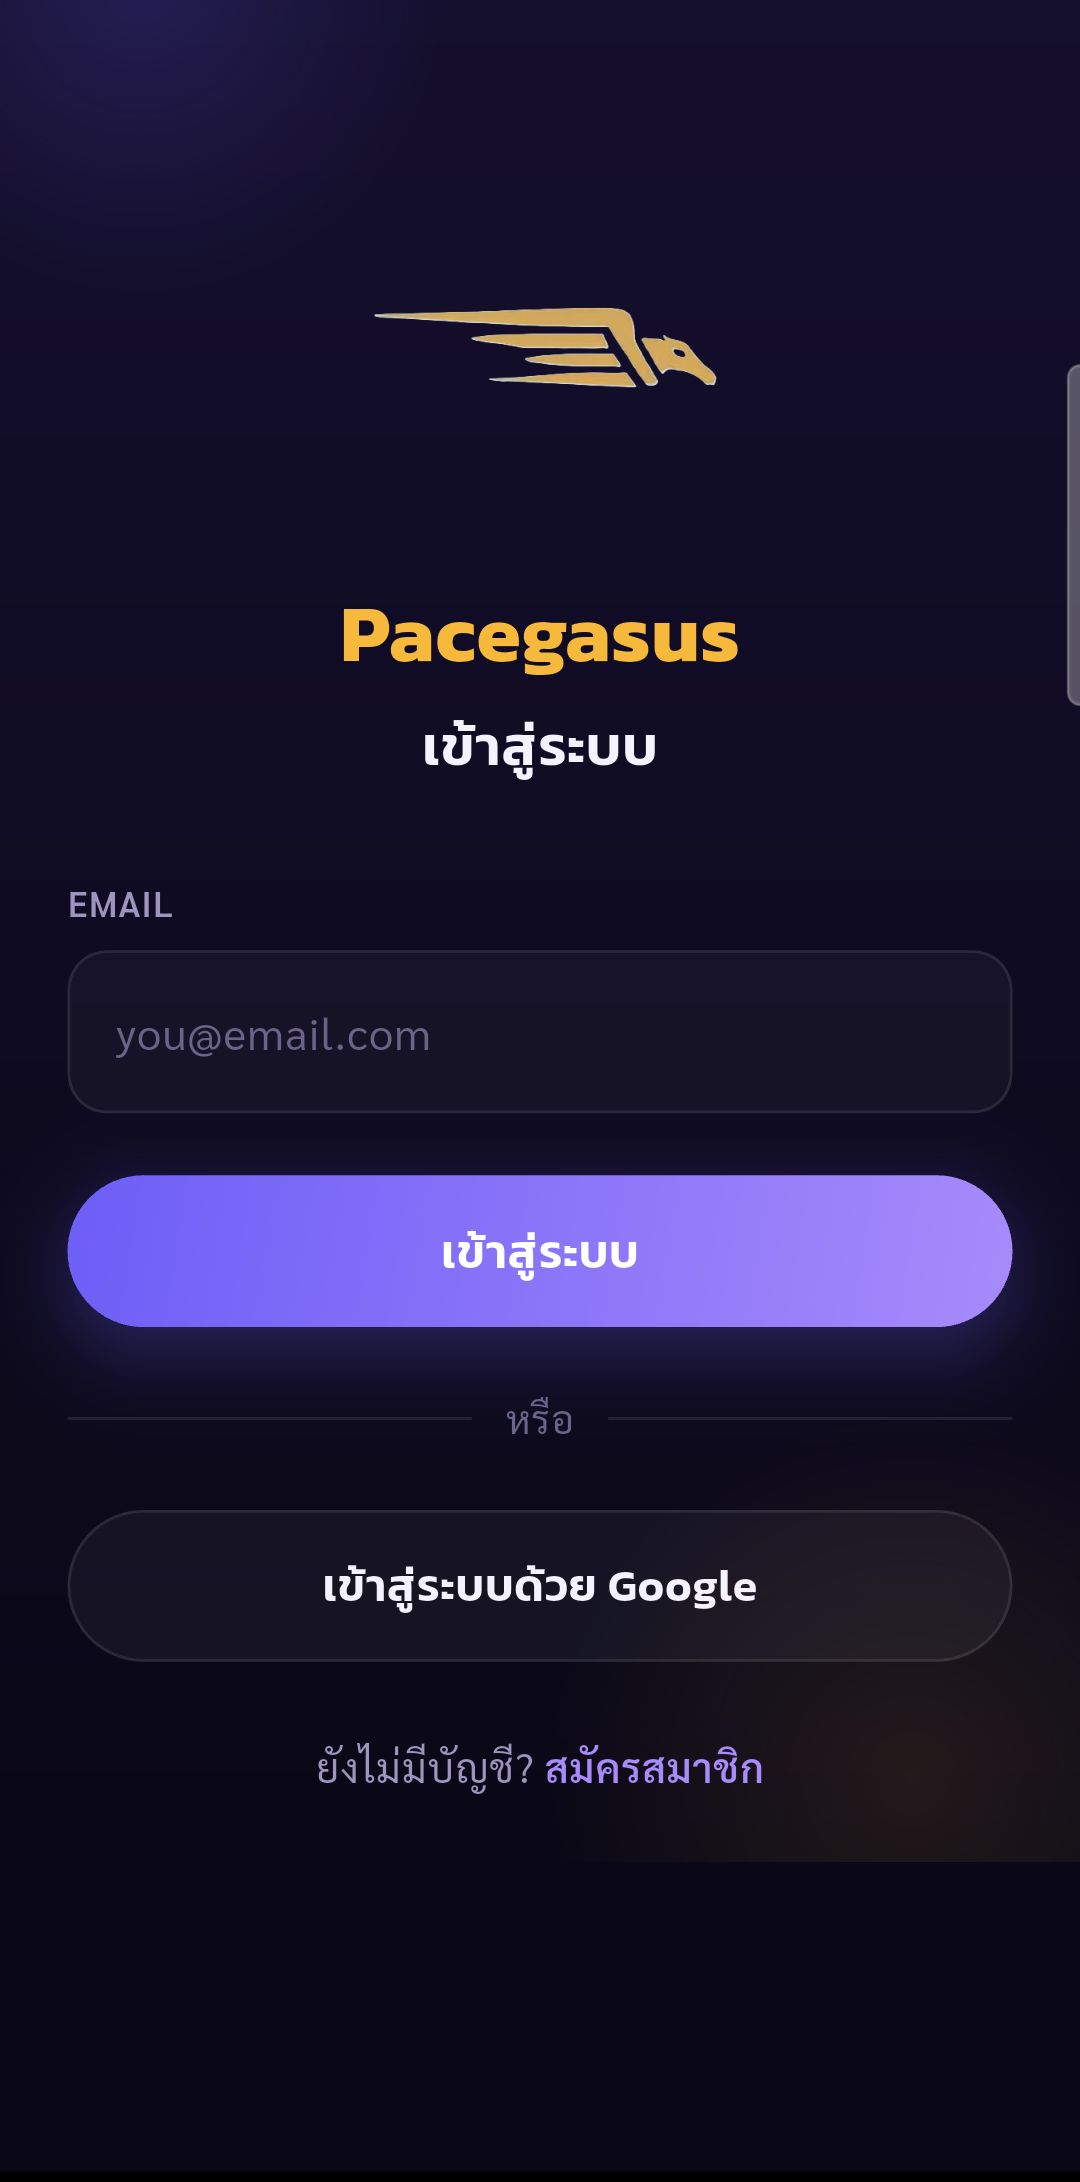
\includegraphics[width=\textwidth]{images/pegasus-login.png}\caption{เข้าสู่ระบบ}\end{subfigure}\hfill
\begin{subfigure}[t]{0.31\textwidth}\centering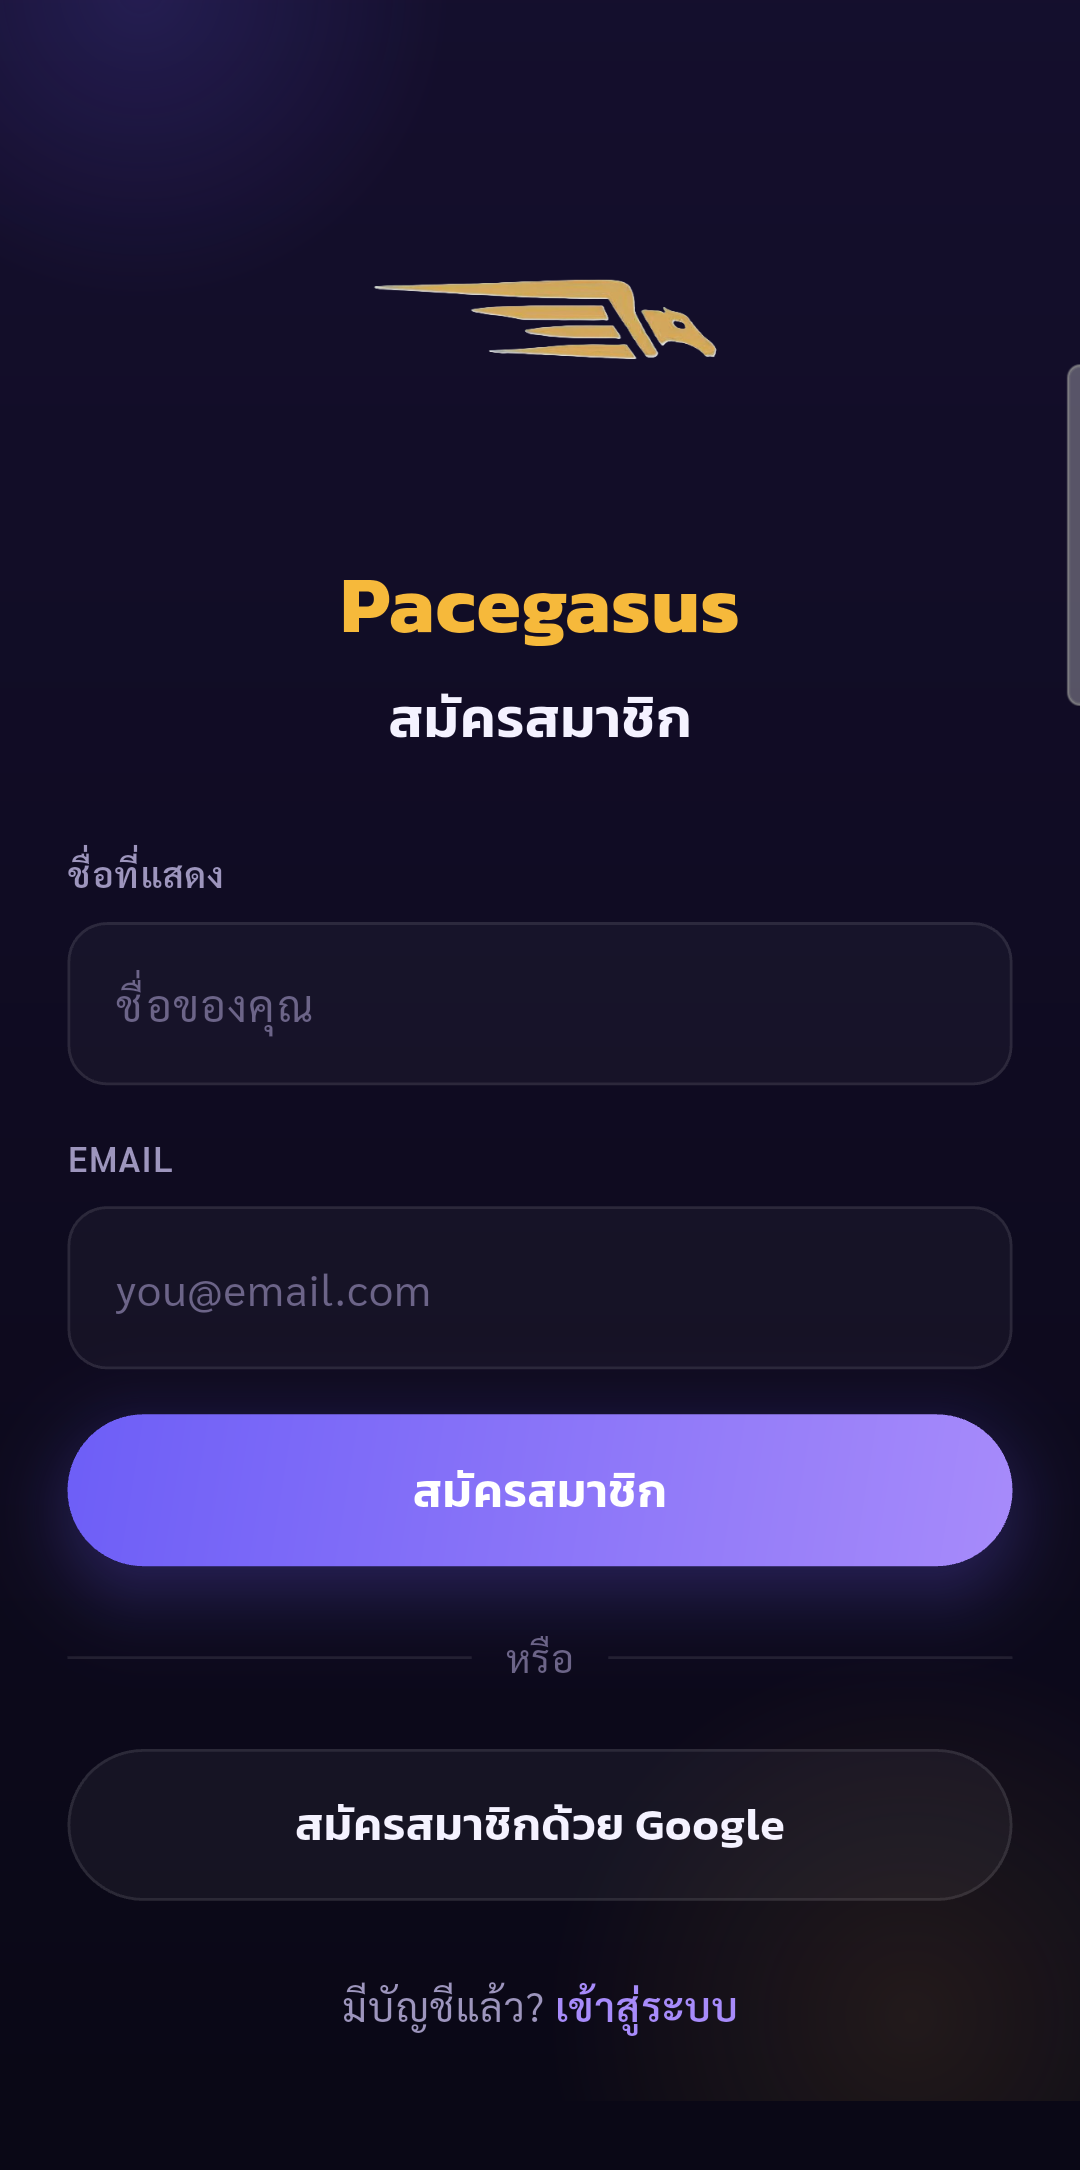
\includegraphics[width=\textwidth]{images/pegasus-sign-up.png}\caption{สมัครสมาชิก}\end{subfigure}\hfill
\begin{subfigure}[t]{0.31\textwidth}\centering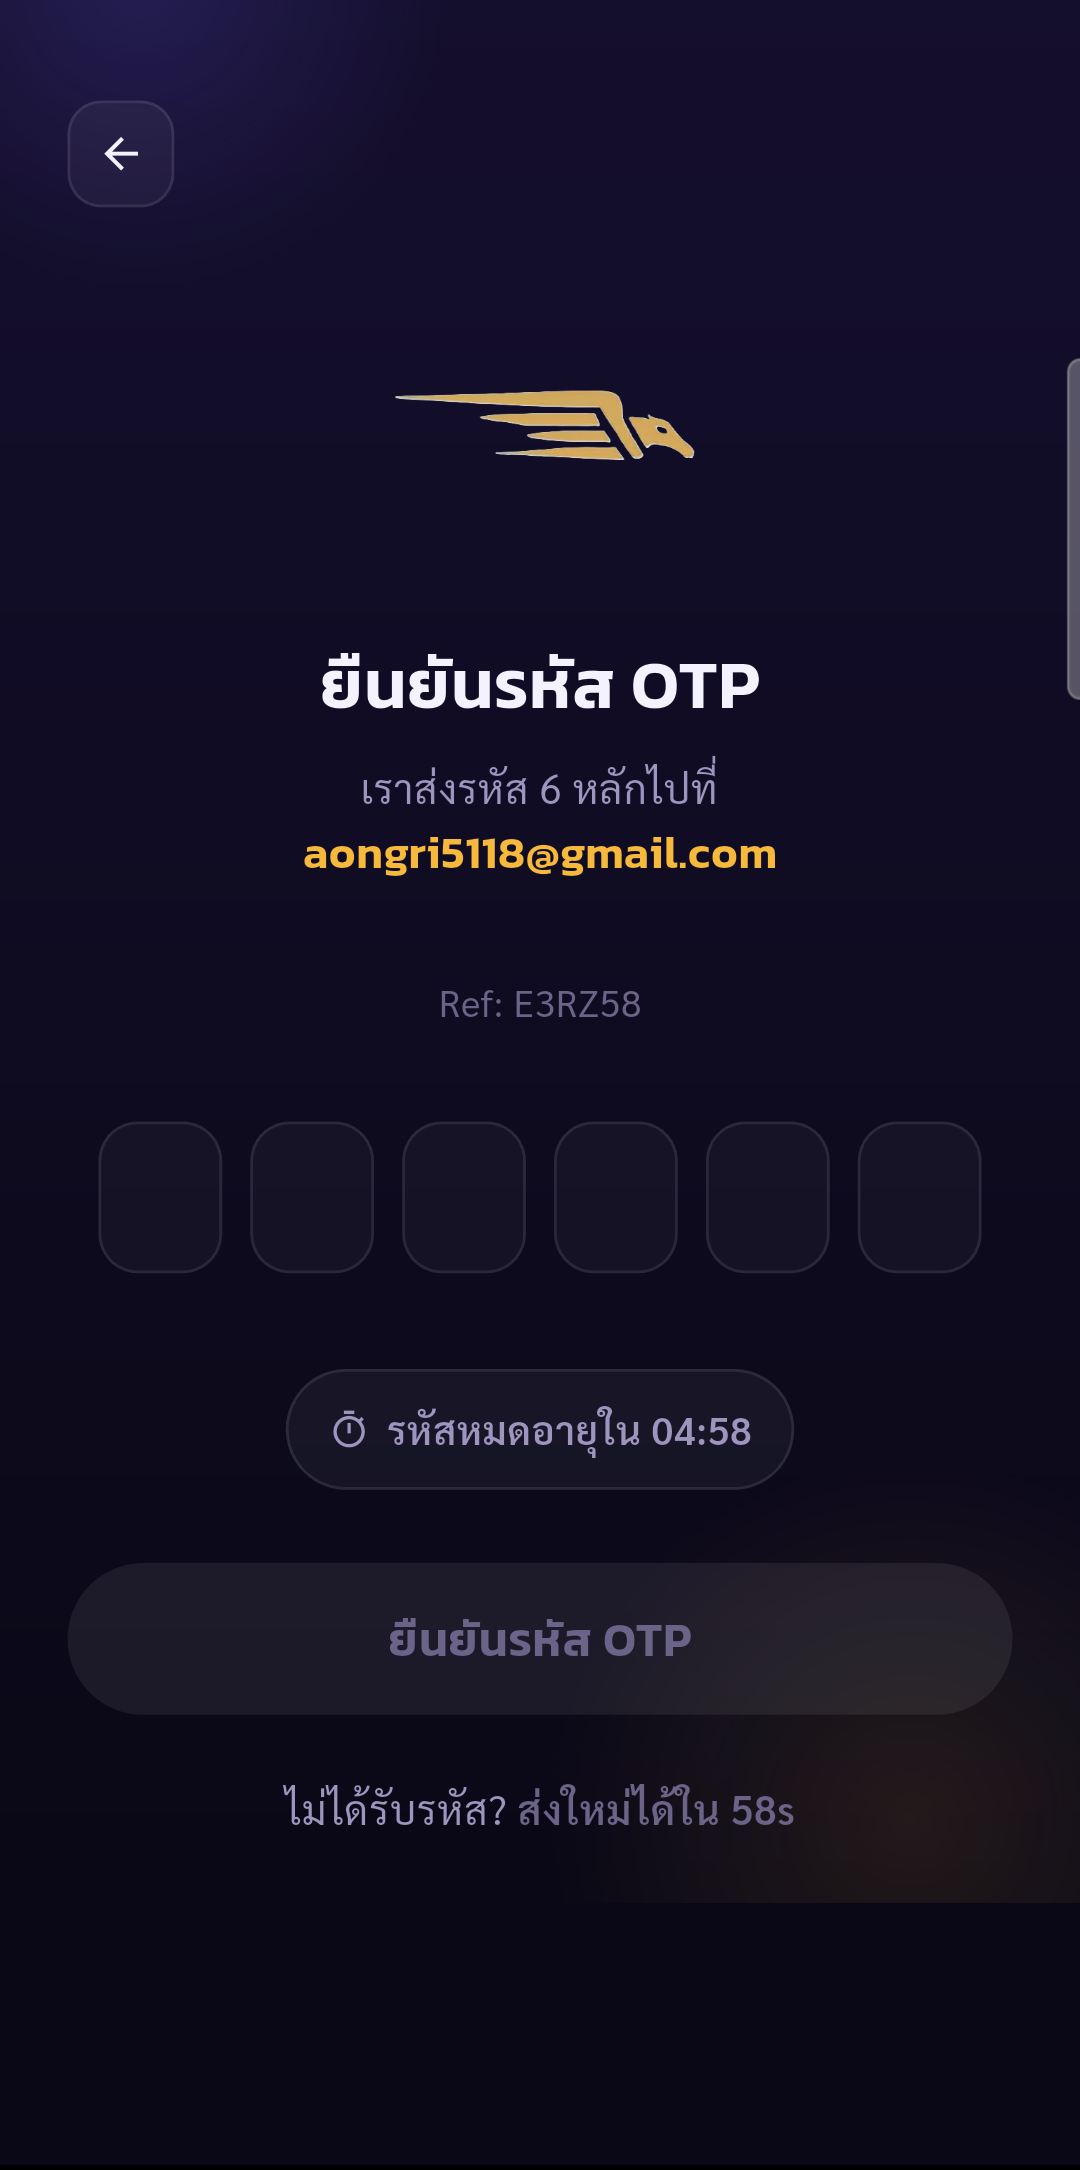
\includegraphics[width=\textwidth]{images/pegasus-otp-verification.png}\caption{ยืนยัน OTP}\end{subfigure}
\caption{หน้าจอการเข้าสู่ระบบและการสมัครสมาชิก}\label{fig:app-auth}
\end{figure}

\begin{figure}[H]\centering
\begin{subfigure}[t]{0.31\textwidth}\centering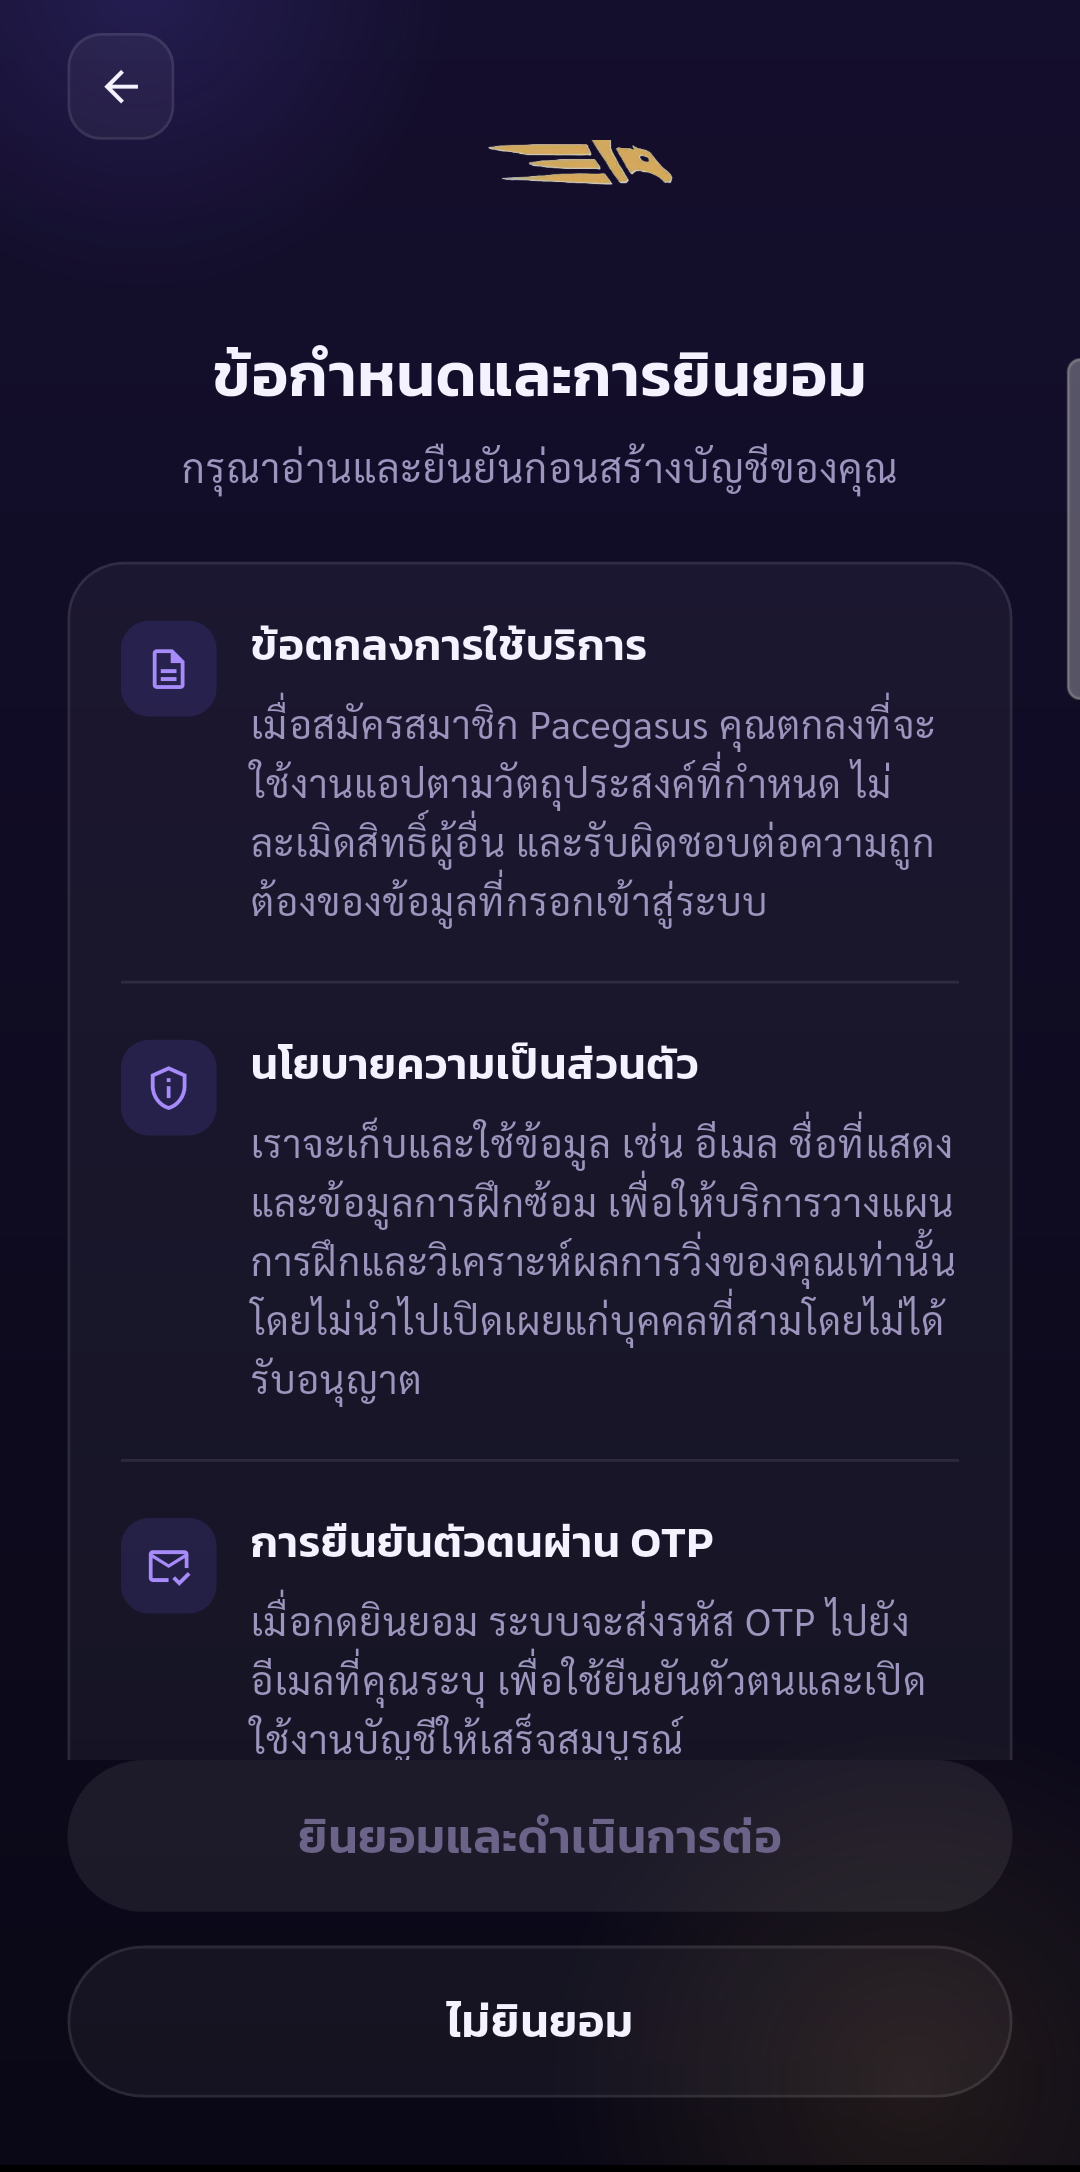
\includegraphics[width=\textwidth]{images/pegasus-terms-and-consent-unchecked.png}\caption{ยังไม่ยินยอม}\end{subfigure}\hfill
\begin{subfigure}[t]{0.31\textwidth}\centering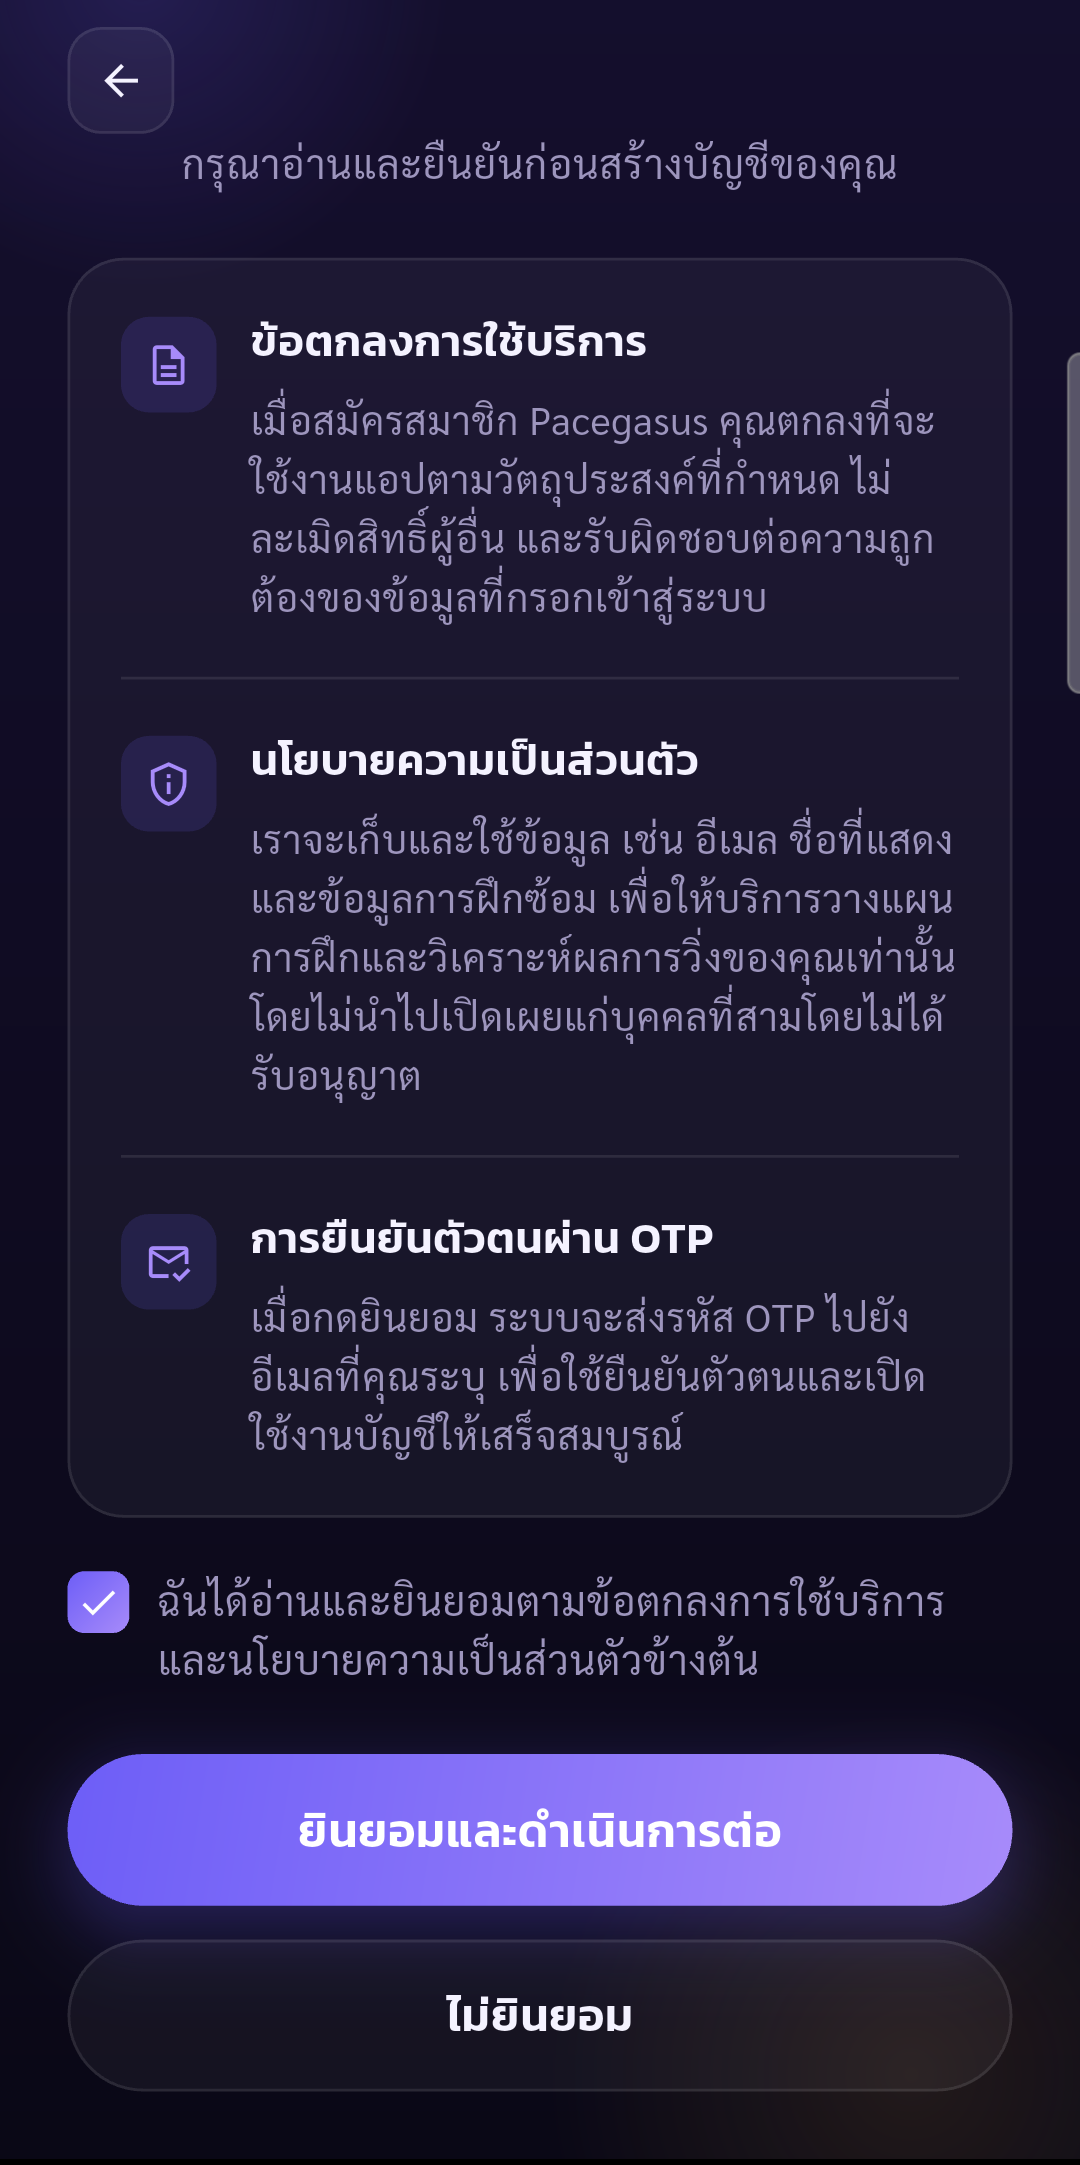
\includegraphics[width=\textwidth]{images/pegasus-terms-and-consent-checked.png}\caption{ยินยอมแล้ว}\end{subfigure}
\caption{หน้าข้อกำหนดและการยินยอม}\label{fig:app-consent}
\end{figure}

\subsection*{การเก็บข้อมูลพื้นฐานและข้อมูลสุขภาพ}

ขั้นตอน Onboarding ประกอบด้วยการกรอกข้อมูลพื้นฐาน ประวัติการวิ่ง และข้อมูลสุขภาพ เพื่อให้ระบบนำไปประกอบการวางแผนการฝึก

\begin{figure}[H]\centering
\begin{subfigure}[t]{0.31\textwidth}\centering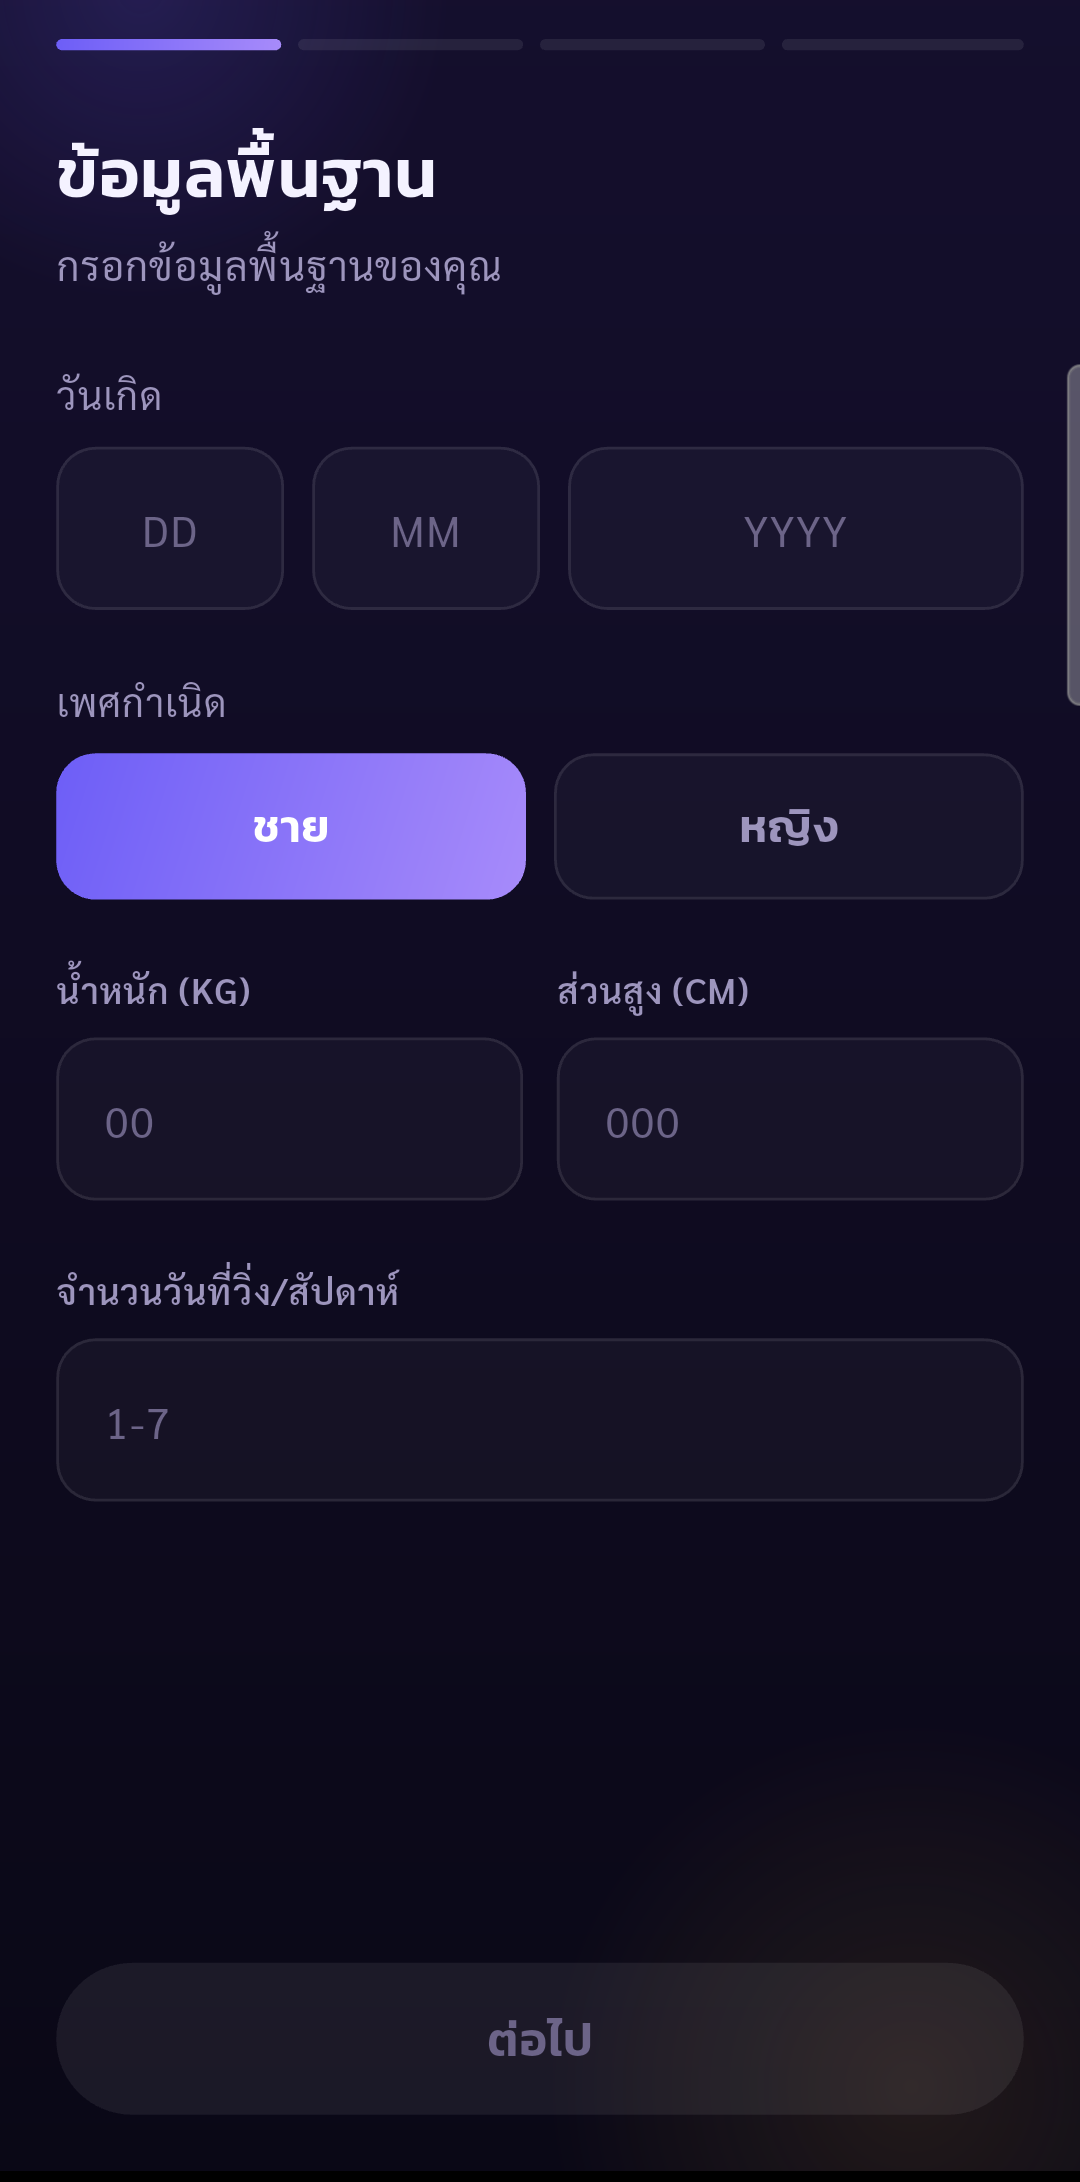
\includegraphics[width=\textwidth]{images/pegasus-onboarding-basic-information.png}\caption{ข้อมูลพื้นฐาน}\end{subfigure}\hfill
\begin{subfigure}[t]{0.31\textwidth}\centering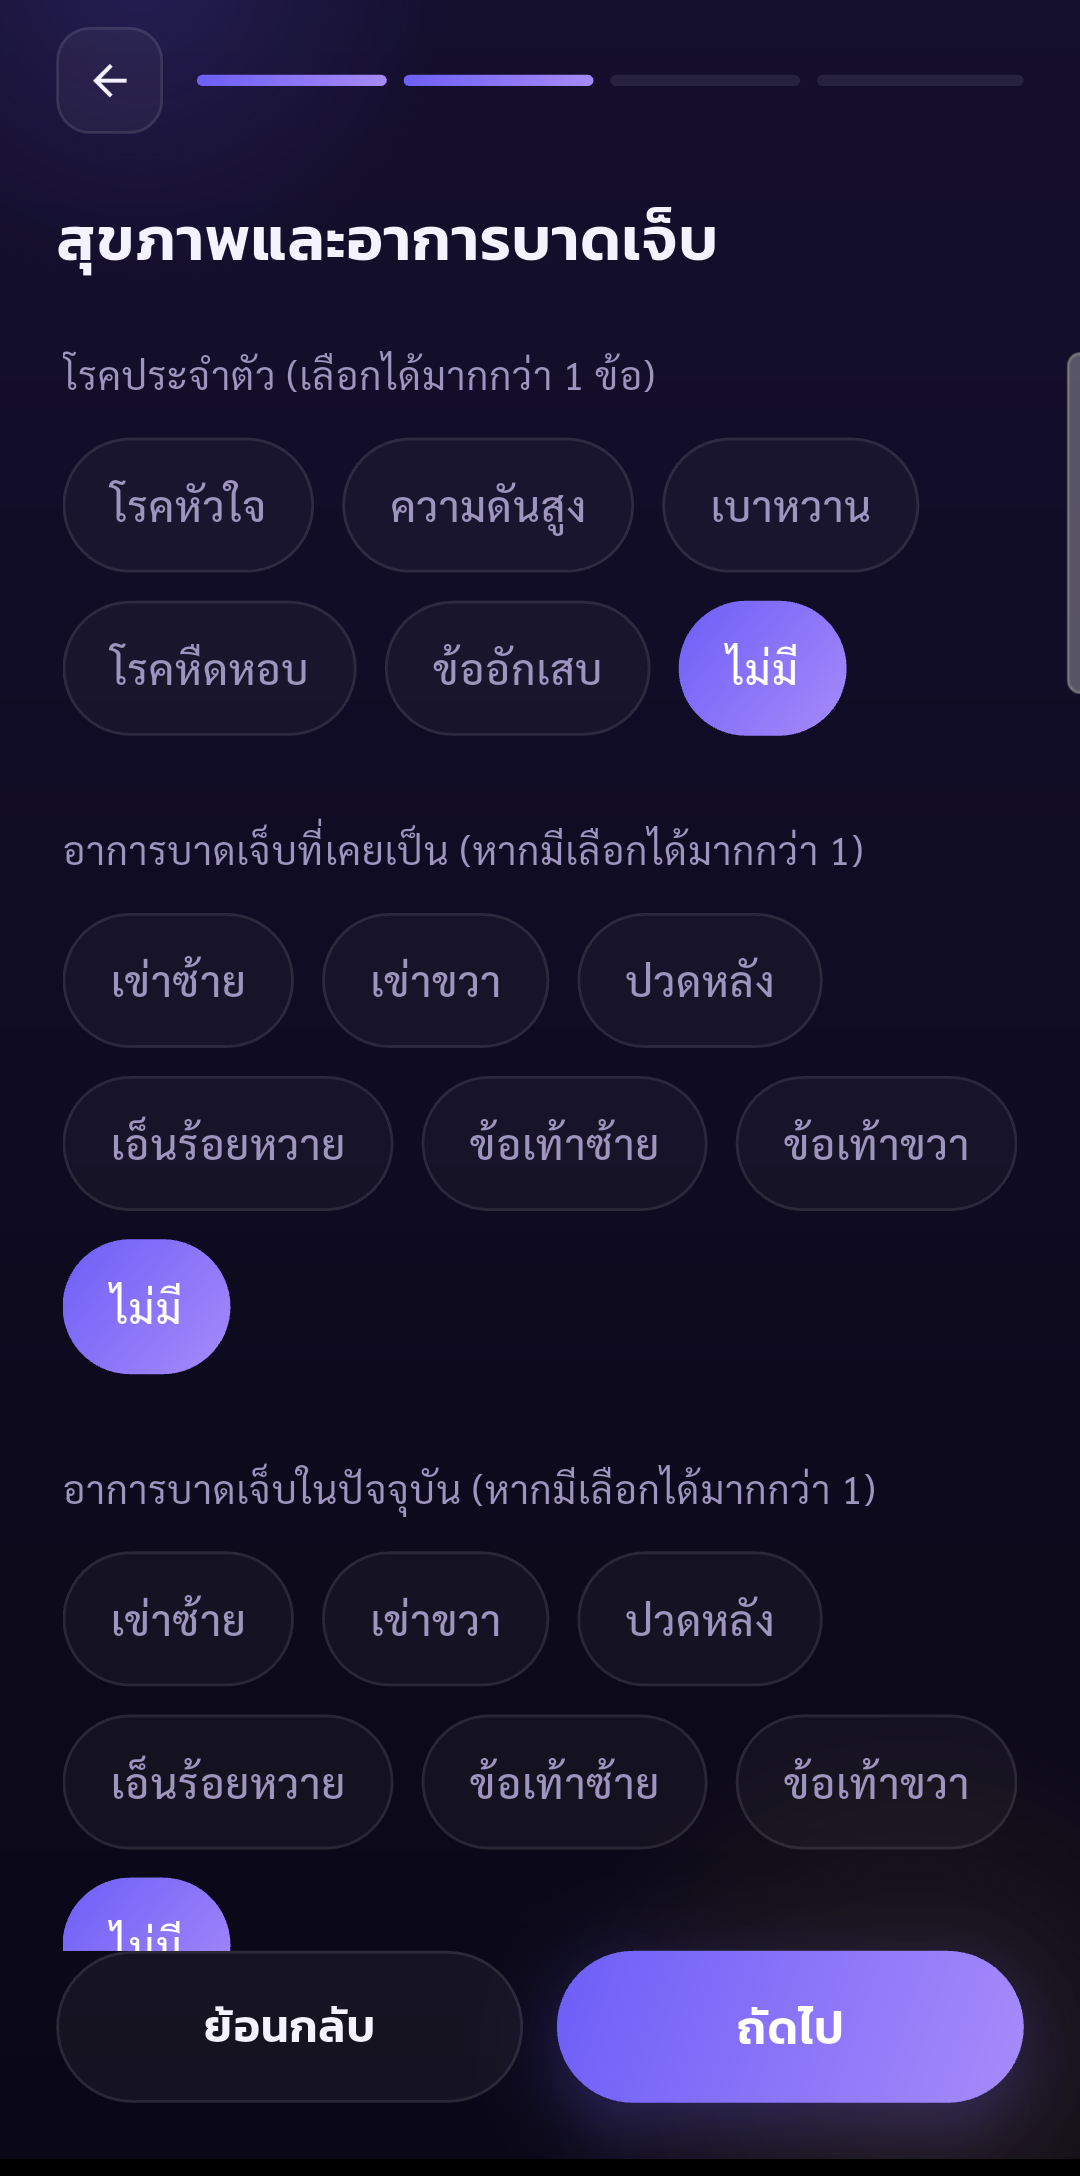
\includegraphics[width=\textwidth]{images/pegasus-onboarding-health-and-injuries.png}\caption{สุขภาพและอาการบาดเจ็บ}\end{subfigure}\hfill
\begin{subfigure}[t]{0.31\textwidth}\centering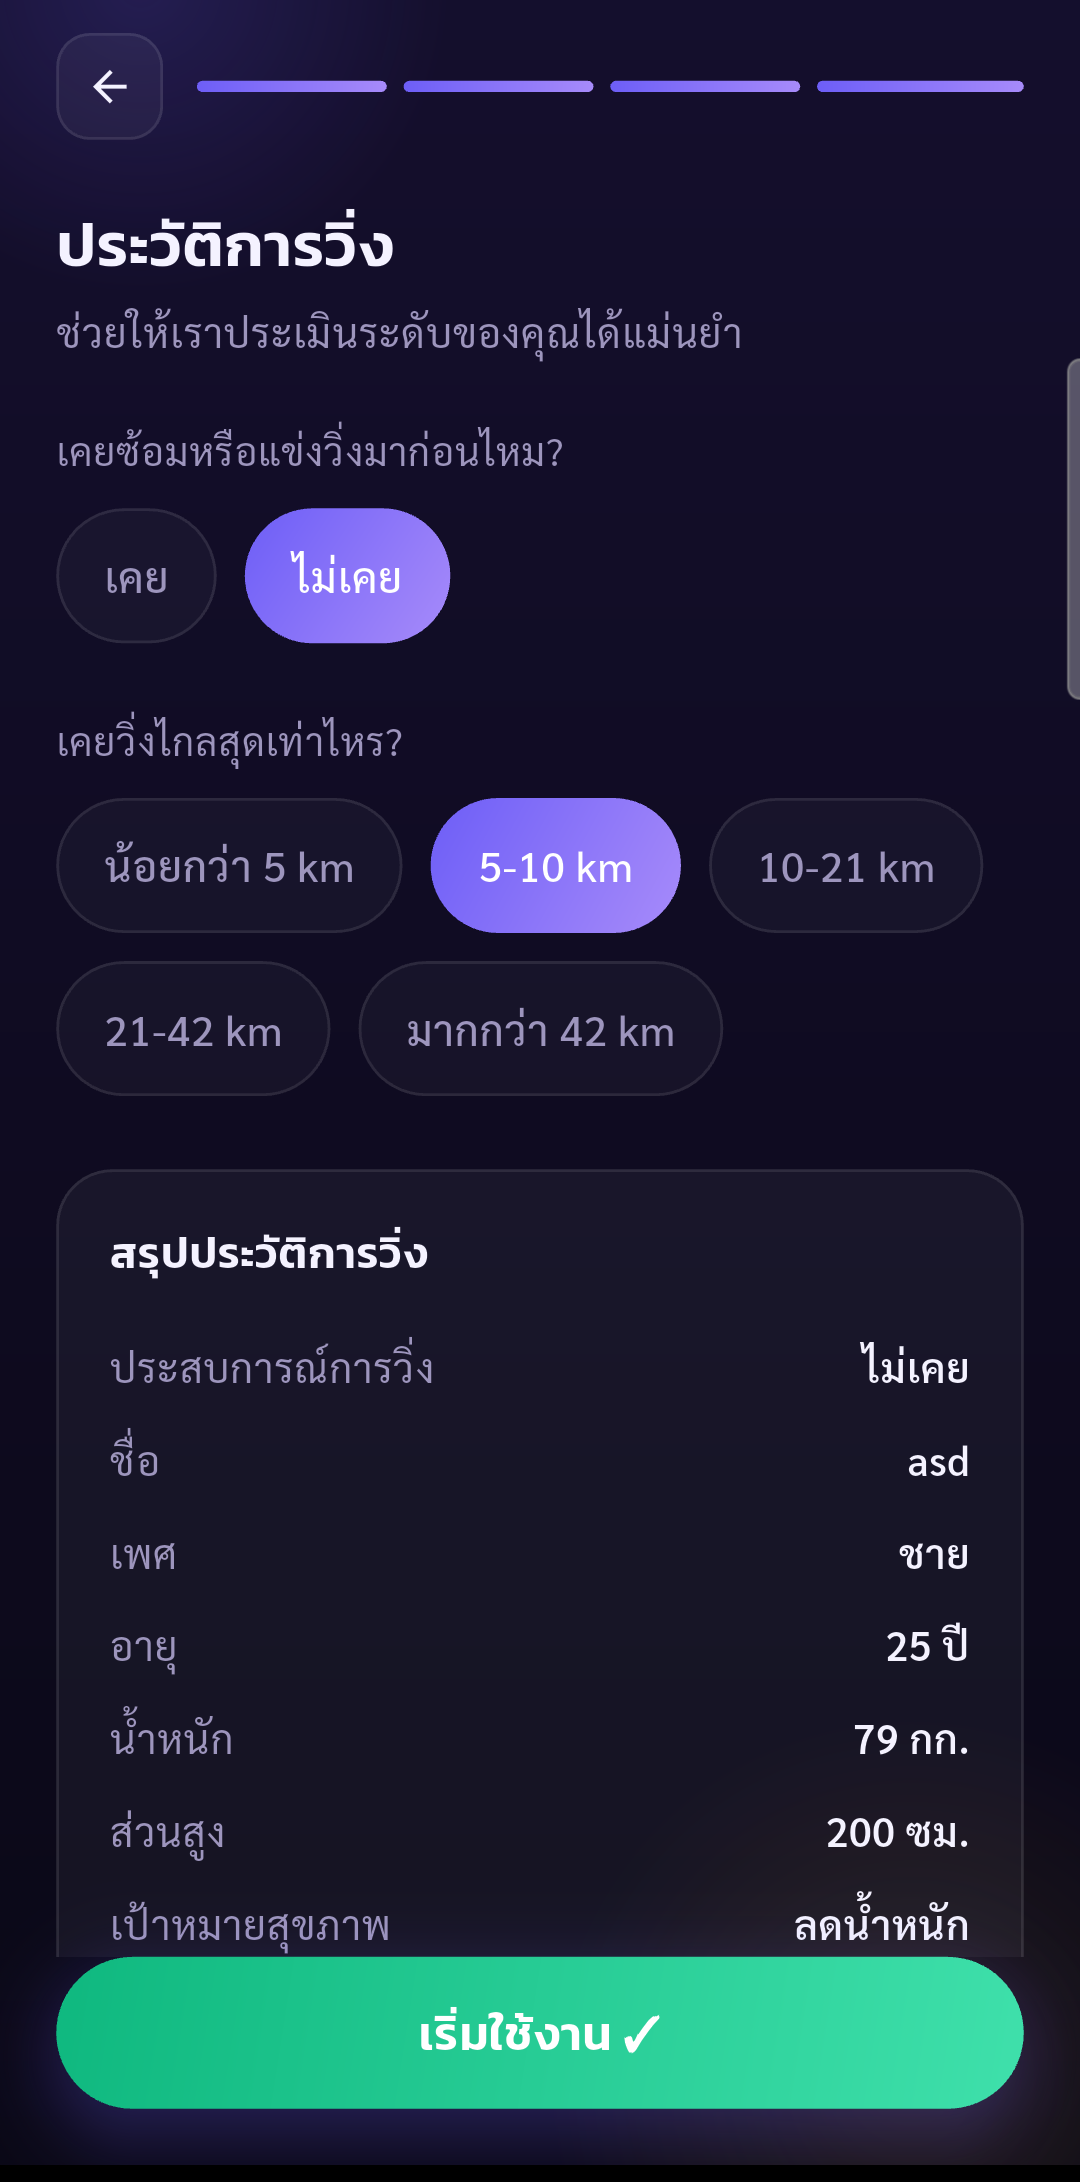
\includegraphics[width=\textwidth]{images/pegasus-onboarding-running-history-summary.png}\caption{ประวัติการวิ่ง}\end{subfigure}
\caption{หน้าจอการเก็บข้อมูลสำหรับสร้างโปรไฟล์ผู้ใช้}\label{fig:app-onboarding}
\end{figure}

\subsection*{การกำหนดเป้าหมายและการเลือกแผนการฝึก}

ผู้ใช้สามารถเลือกเป้าหมายด้านระยะทางและเป้าหมายด้านสุขภาพ ระบบจะใช้ข้อมูลดังกล่าวเป็นเงื่อนไขเริ่มต้นของ Adaptive Training Engine

\begin{figure}[H]\centering
\begin{subfigure}[t]{0.31\textwidth}\centering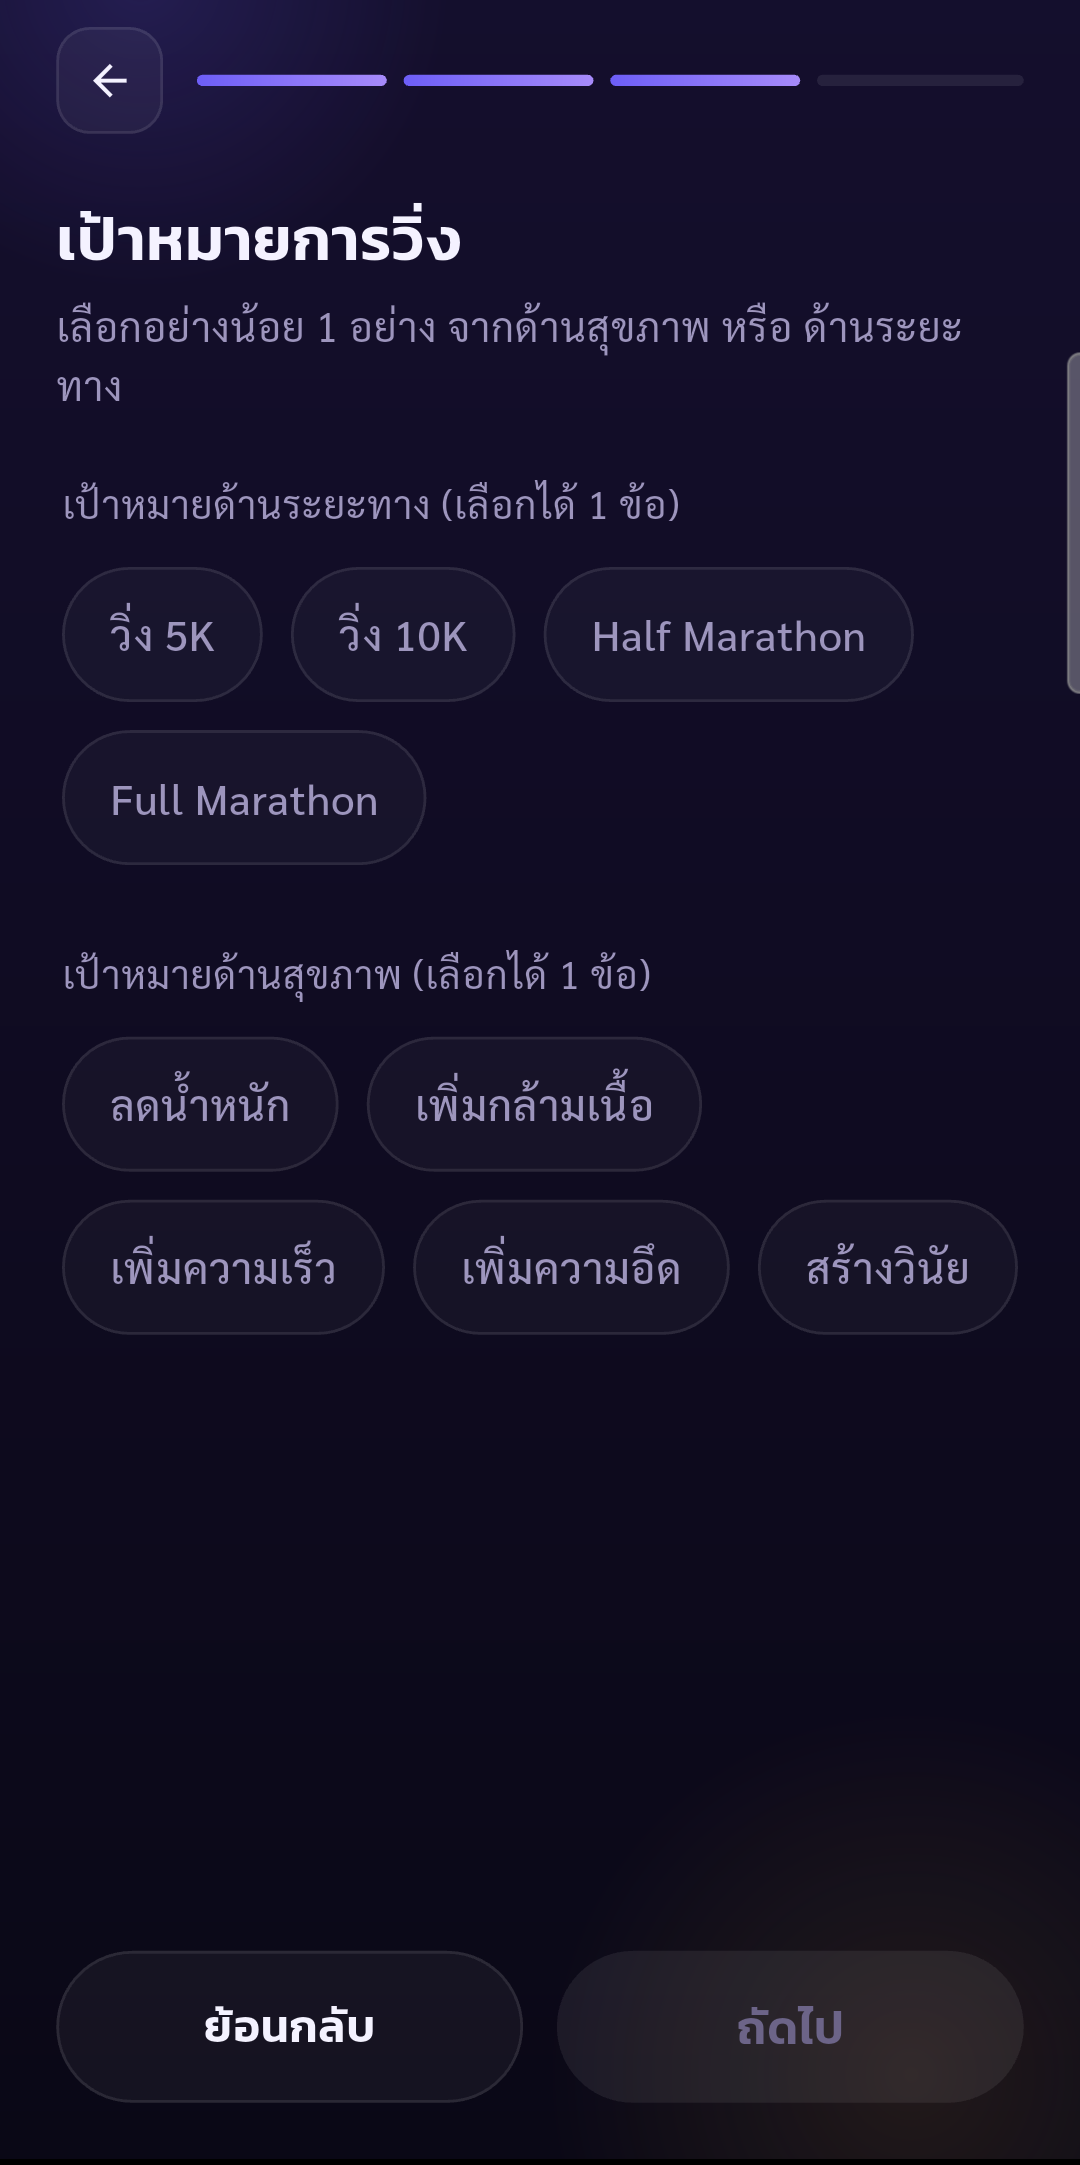
\includegraphics[width=\textwidth]{images/pegasus-onboarding-running-goals.png}\caption{เป้าหมายการวิ่ง}\end{subfigure}\hfill
\begin{subfigure}[t]{0.31\textwidth}\centering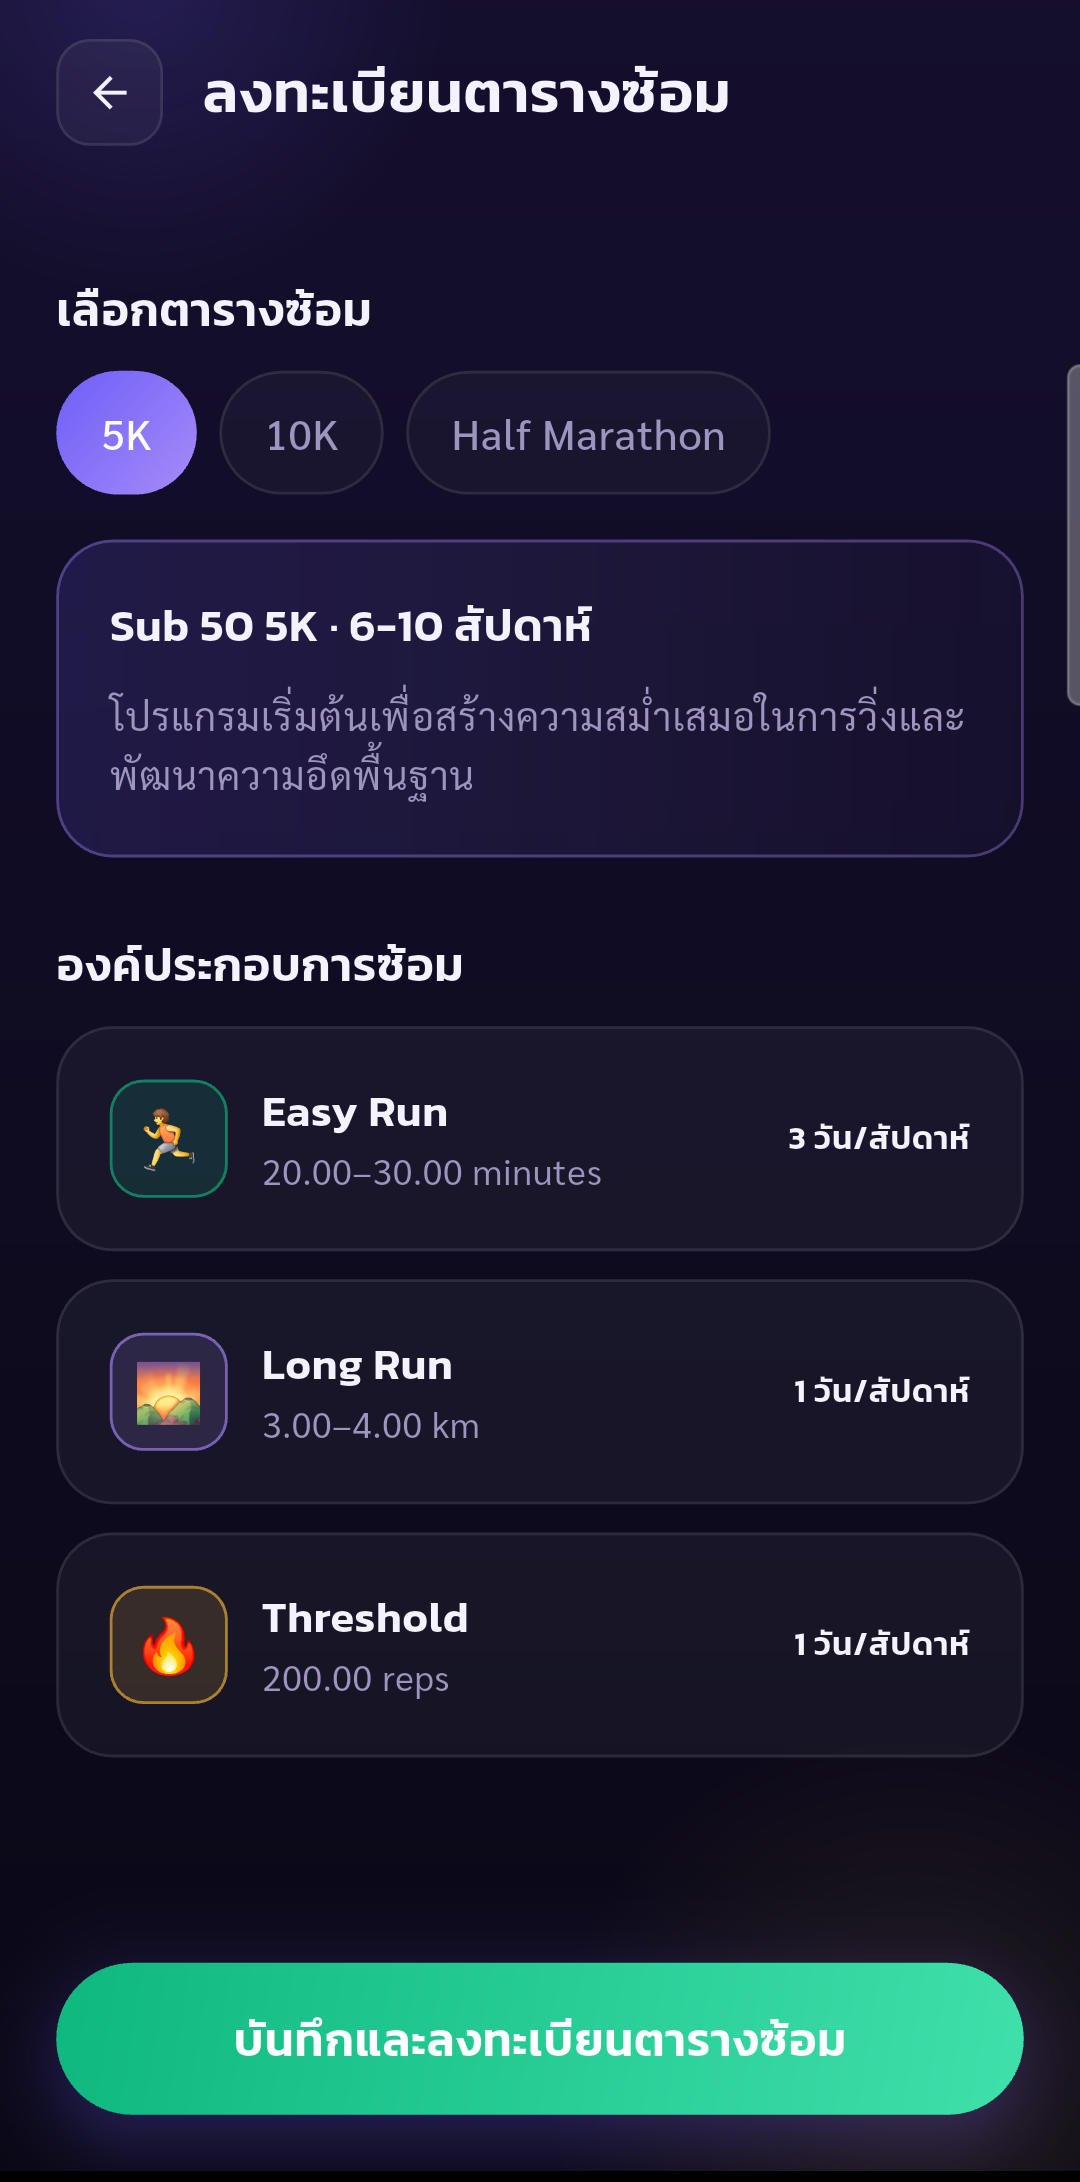
\includegraphics[width=\textwidth]{images/pegasus-training-plan-5k.png}\caption{แผน 5K}\end{subfigure}\hfill
\begin{subfigure}[t]{0.31\textwidth}\centering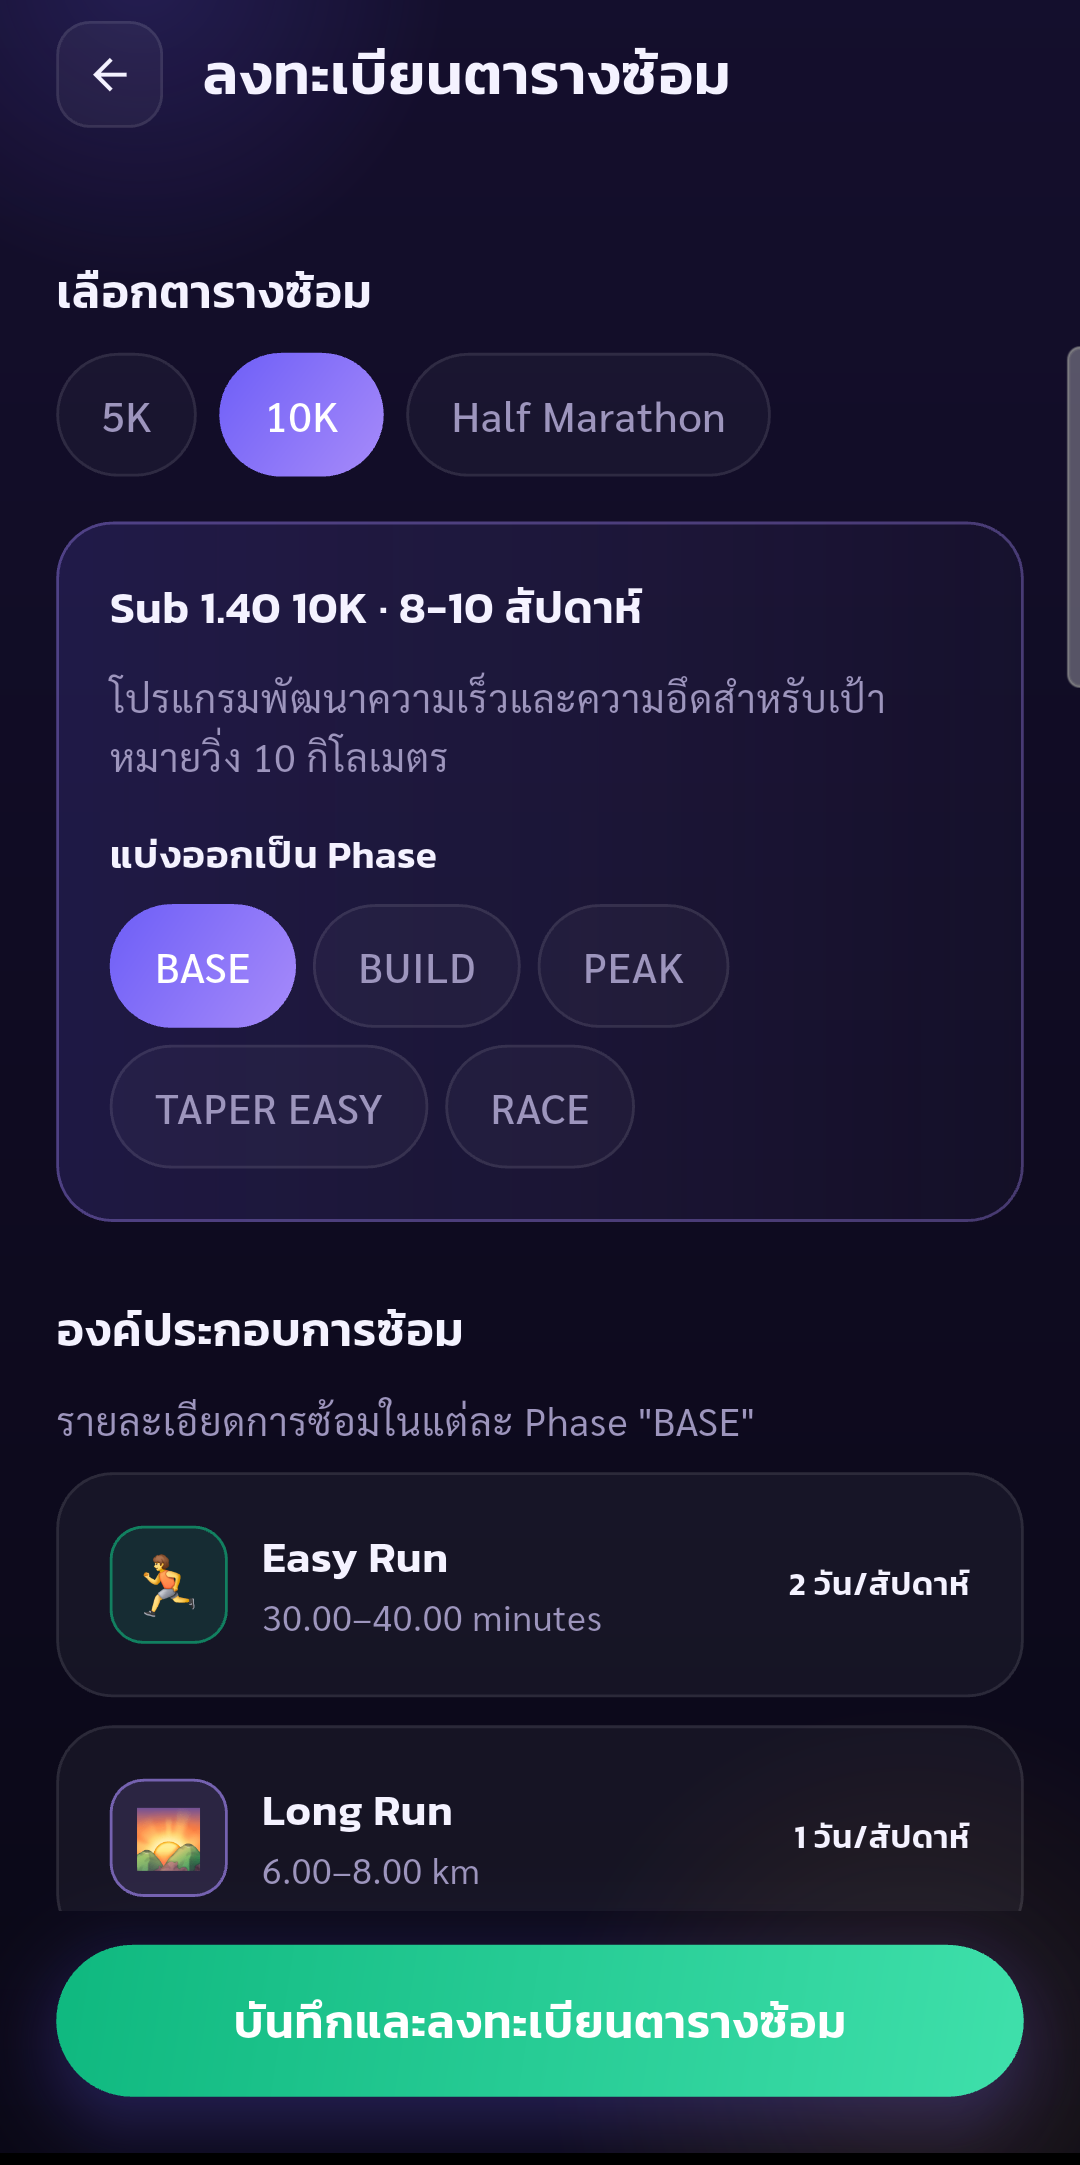
\includegraphics[width=\textwidth]{images/pegasus-training-plan-10k.png}\caption{แผน 10K}\end{subfigure}
\caption{การกำหนดเป้าหมายและการเลือกแผนการฝึก}\label{fig:app-goals}
\end{figure}

\begin{figure}[H]\centering
\begin{subfigure}[t]{0.31\textwidth}\centering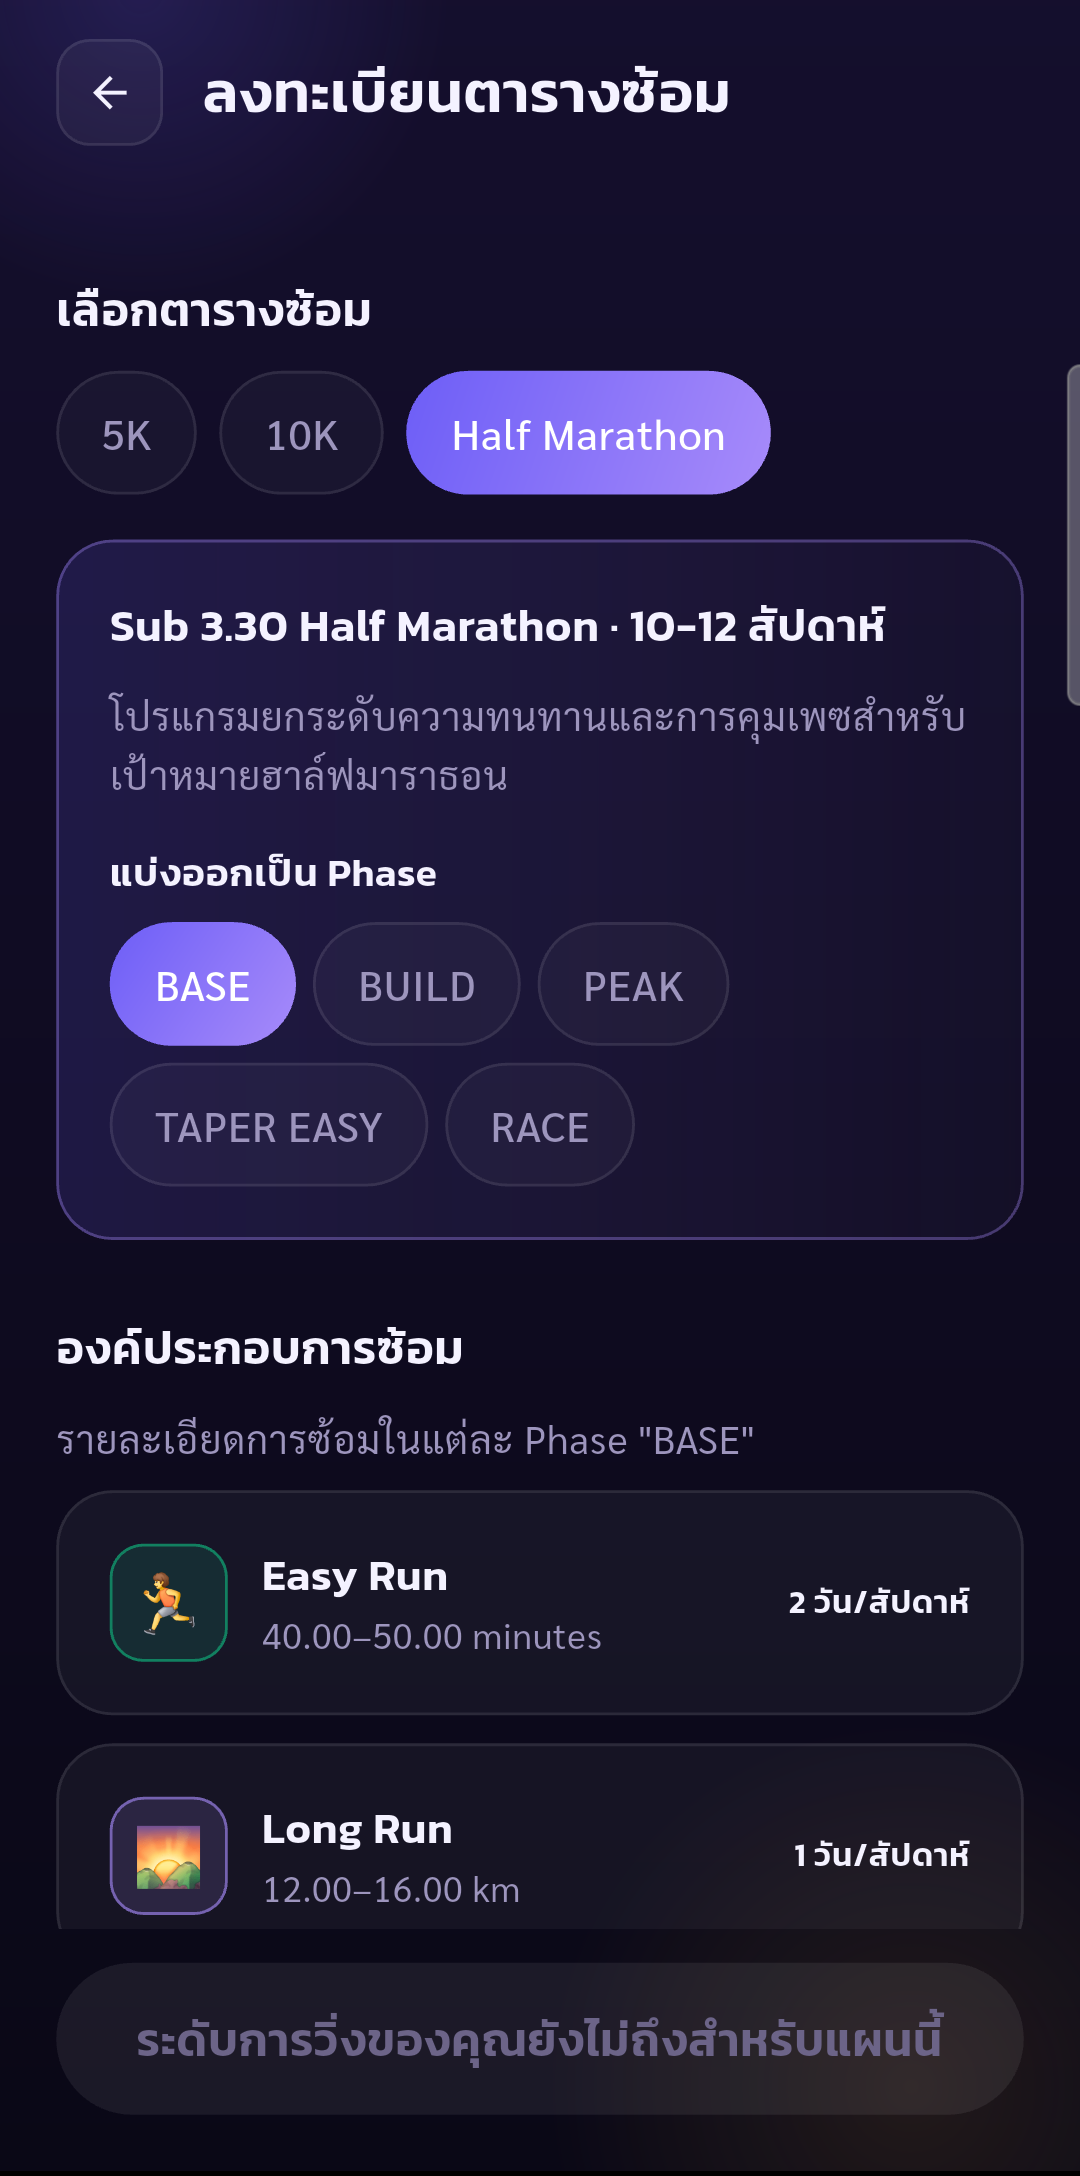
\includegraphics[width=\textwidth]{images/pegasus-training-plan-half-marathon.png}\caption{แผน Half Marathon}\end{subfigure}\hfill
\begin{subfigure}[t]{0.31\textwidth}\centering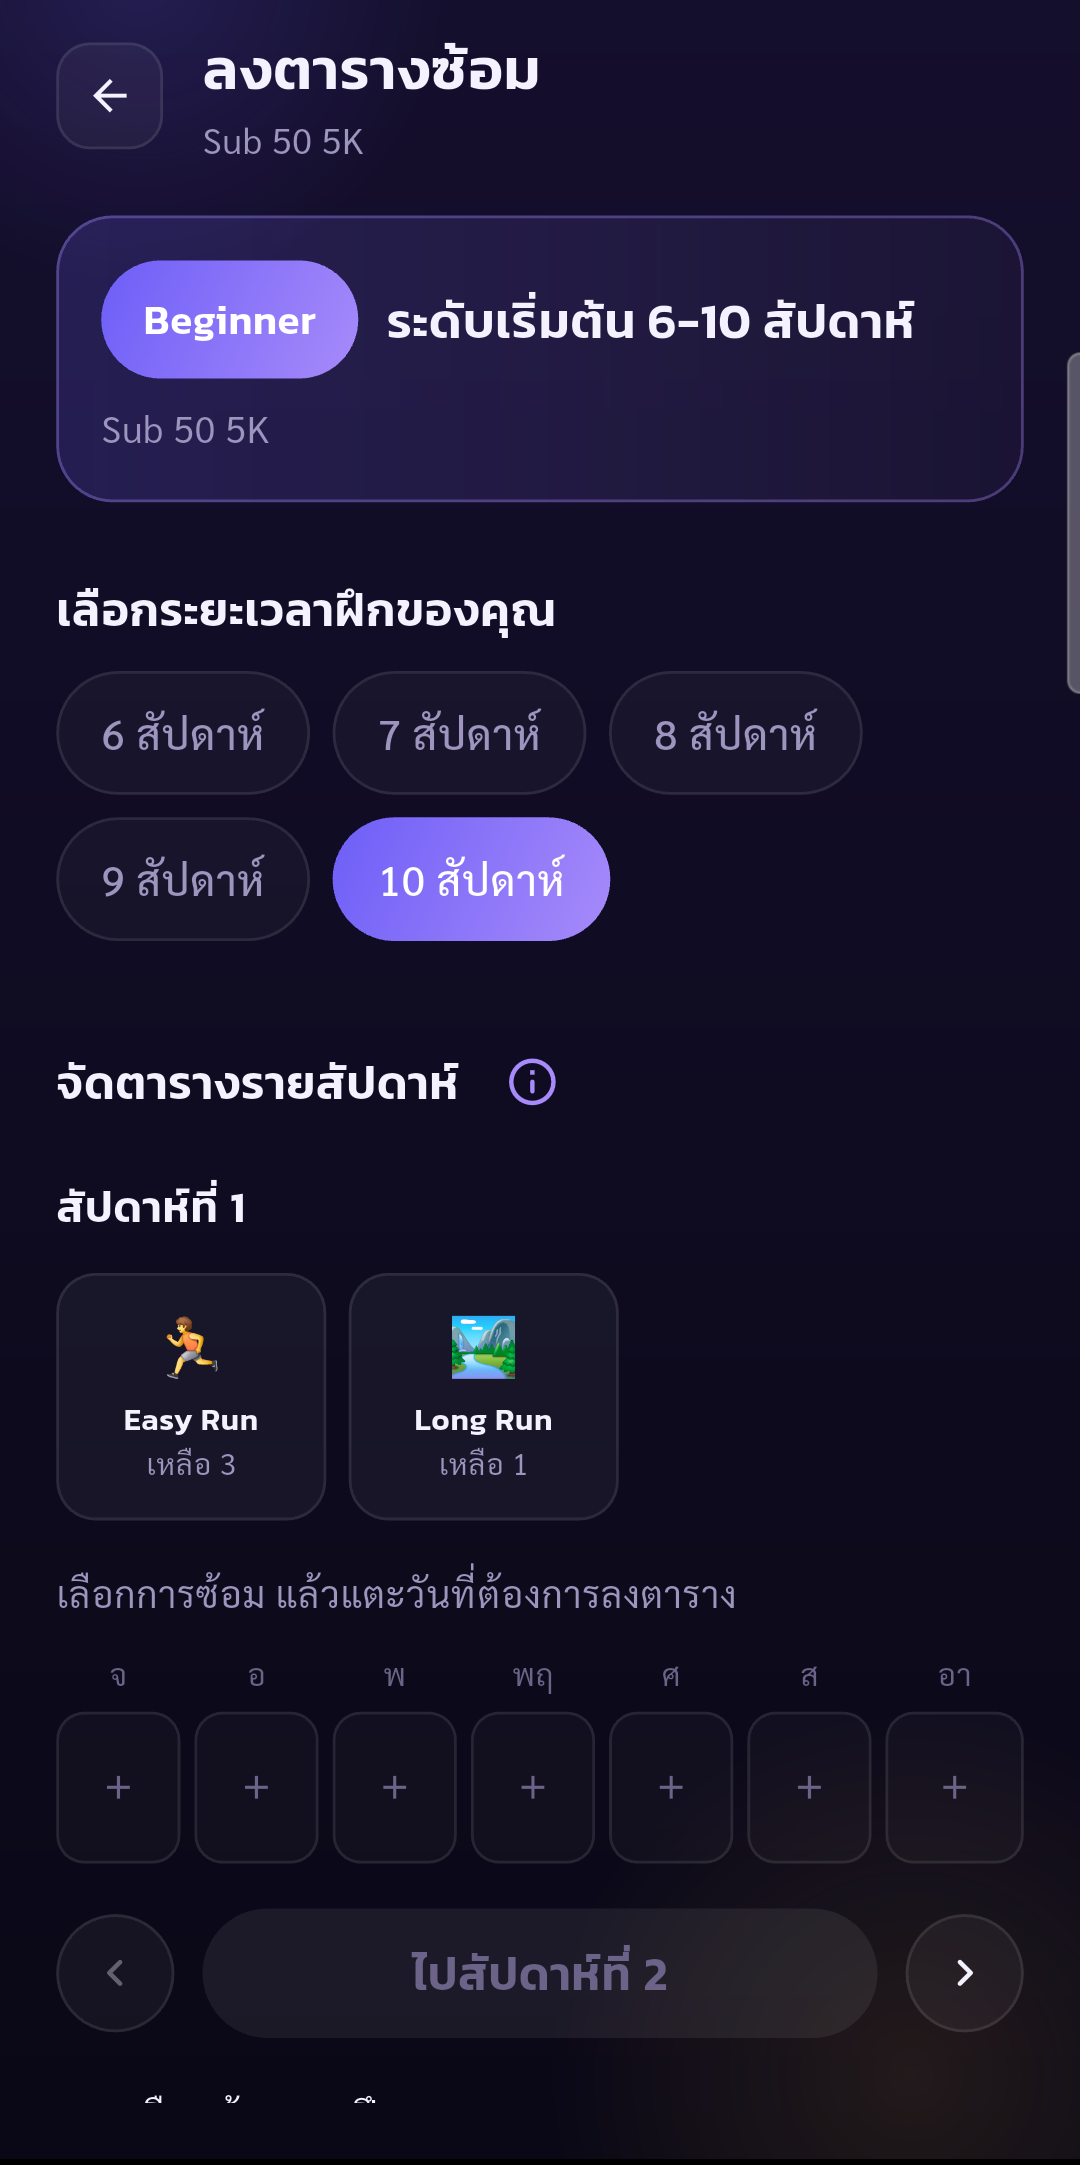
\includegraphics[width=\textwidth]{images/pegasus-schedule-builder-5k.png}\caption{จัดตารางแผน 5K}\end{subfigure}\hfill
\begin{subfigure}[t]{0.31\textwidth}\centering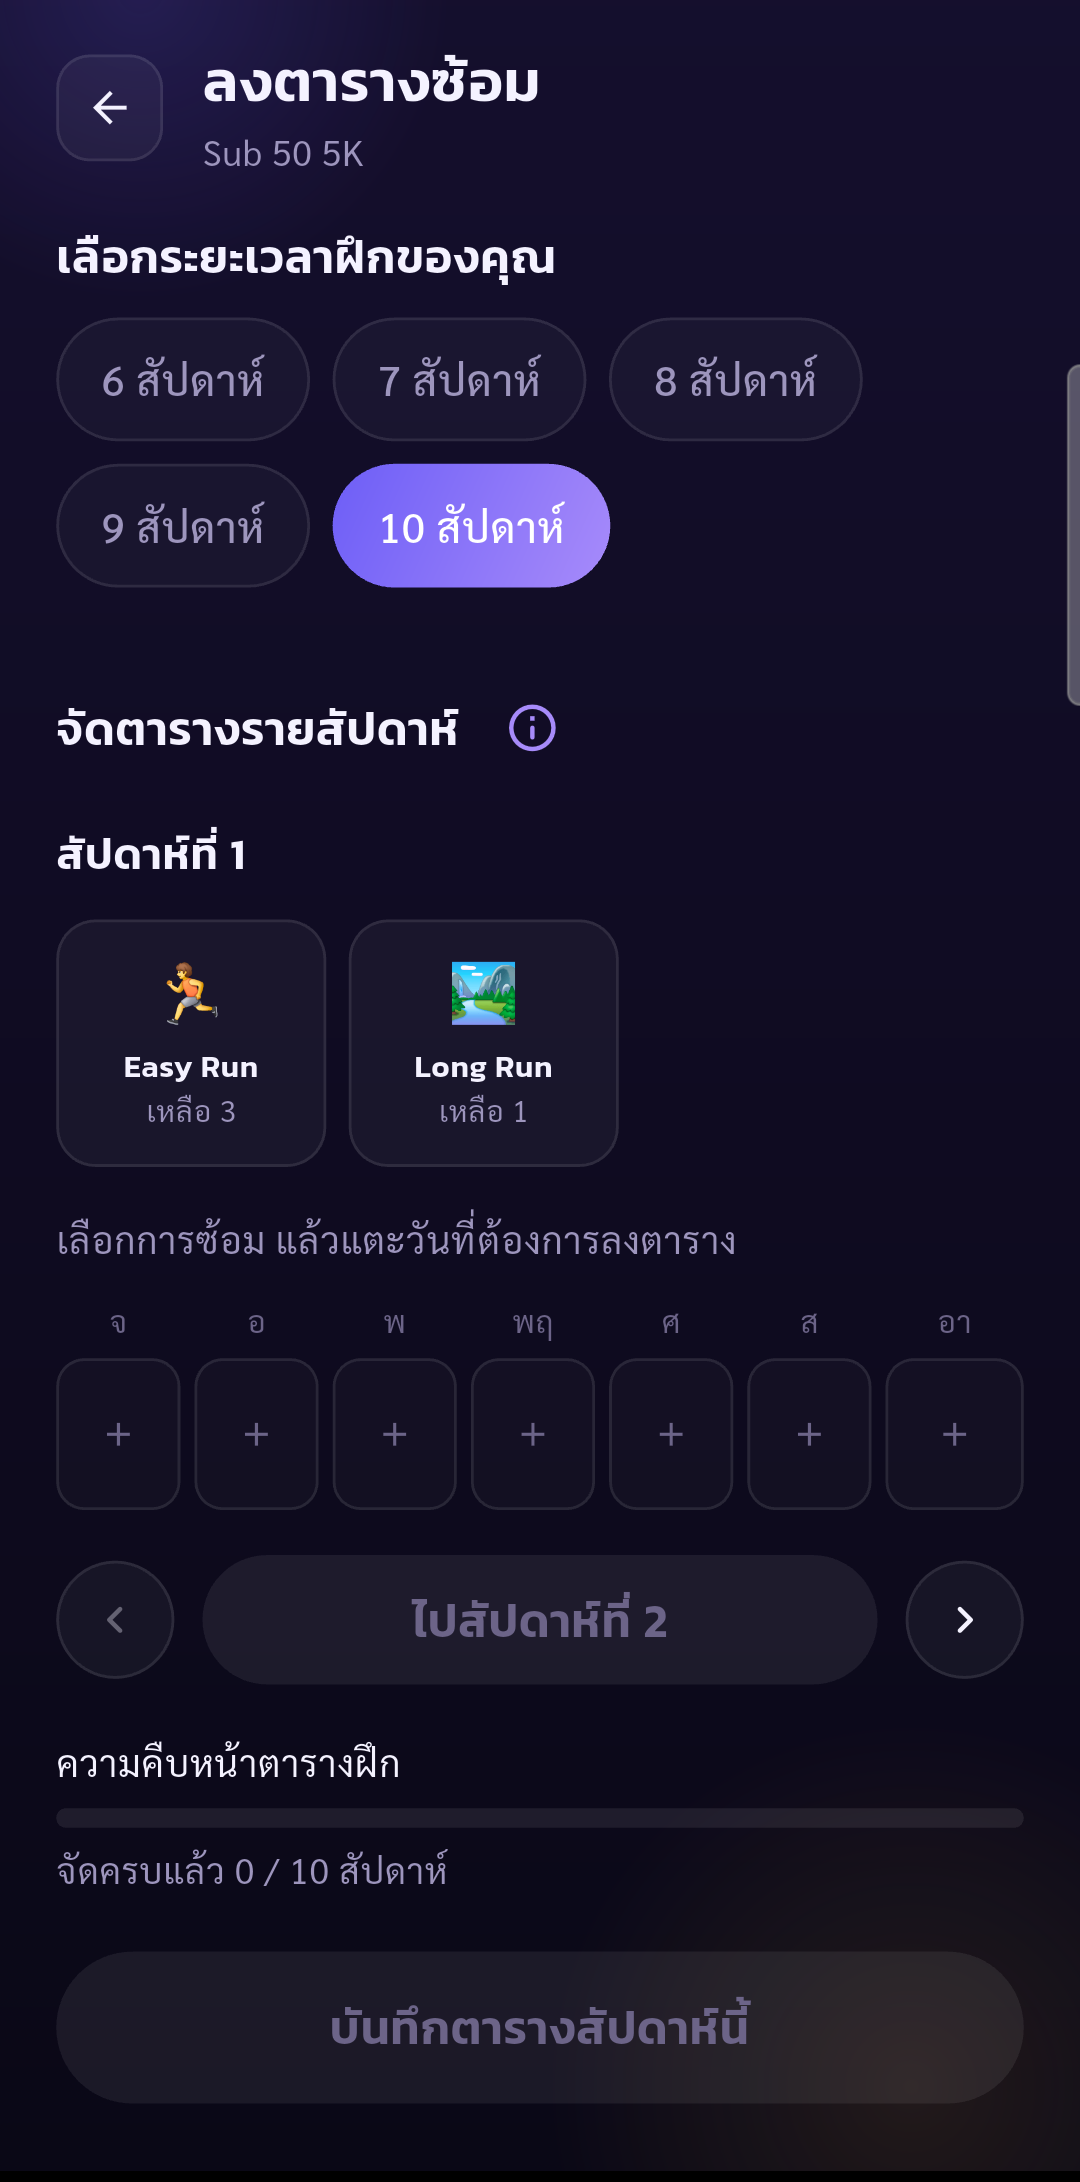
\includegraphics[width=\textwidth]{images/pegasus-schedule-builder-progress.png}\caption{ความคืบหน้าตารางฝึก}\end{subfigure}
\caption{รายละเอียดแผนการฝึกและการจัดตารางรายสัปดาห์}\label{fig:app-plans}
\end{figure}

\subsection*{หน้าหลักและ Daily Wellness Check-in}

หน้าหลักแสดงข้อมูลผู้ใช้ คะแนน เหรียญ กิจกรรมที่ต้องทำ Session การวิ่ง และแผนการฝึก ส่วน Daily Wellness Check-in ใช้ประเมินความพร้อมของผู้ใช้ในแต่ละวัน

\begin{figure}[H]\centering
\begin{subfigure}[t]{0.31\textwidth}\centering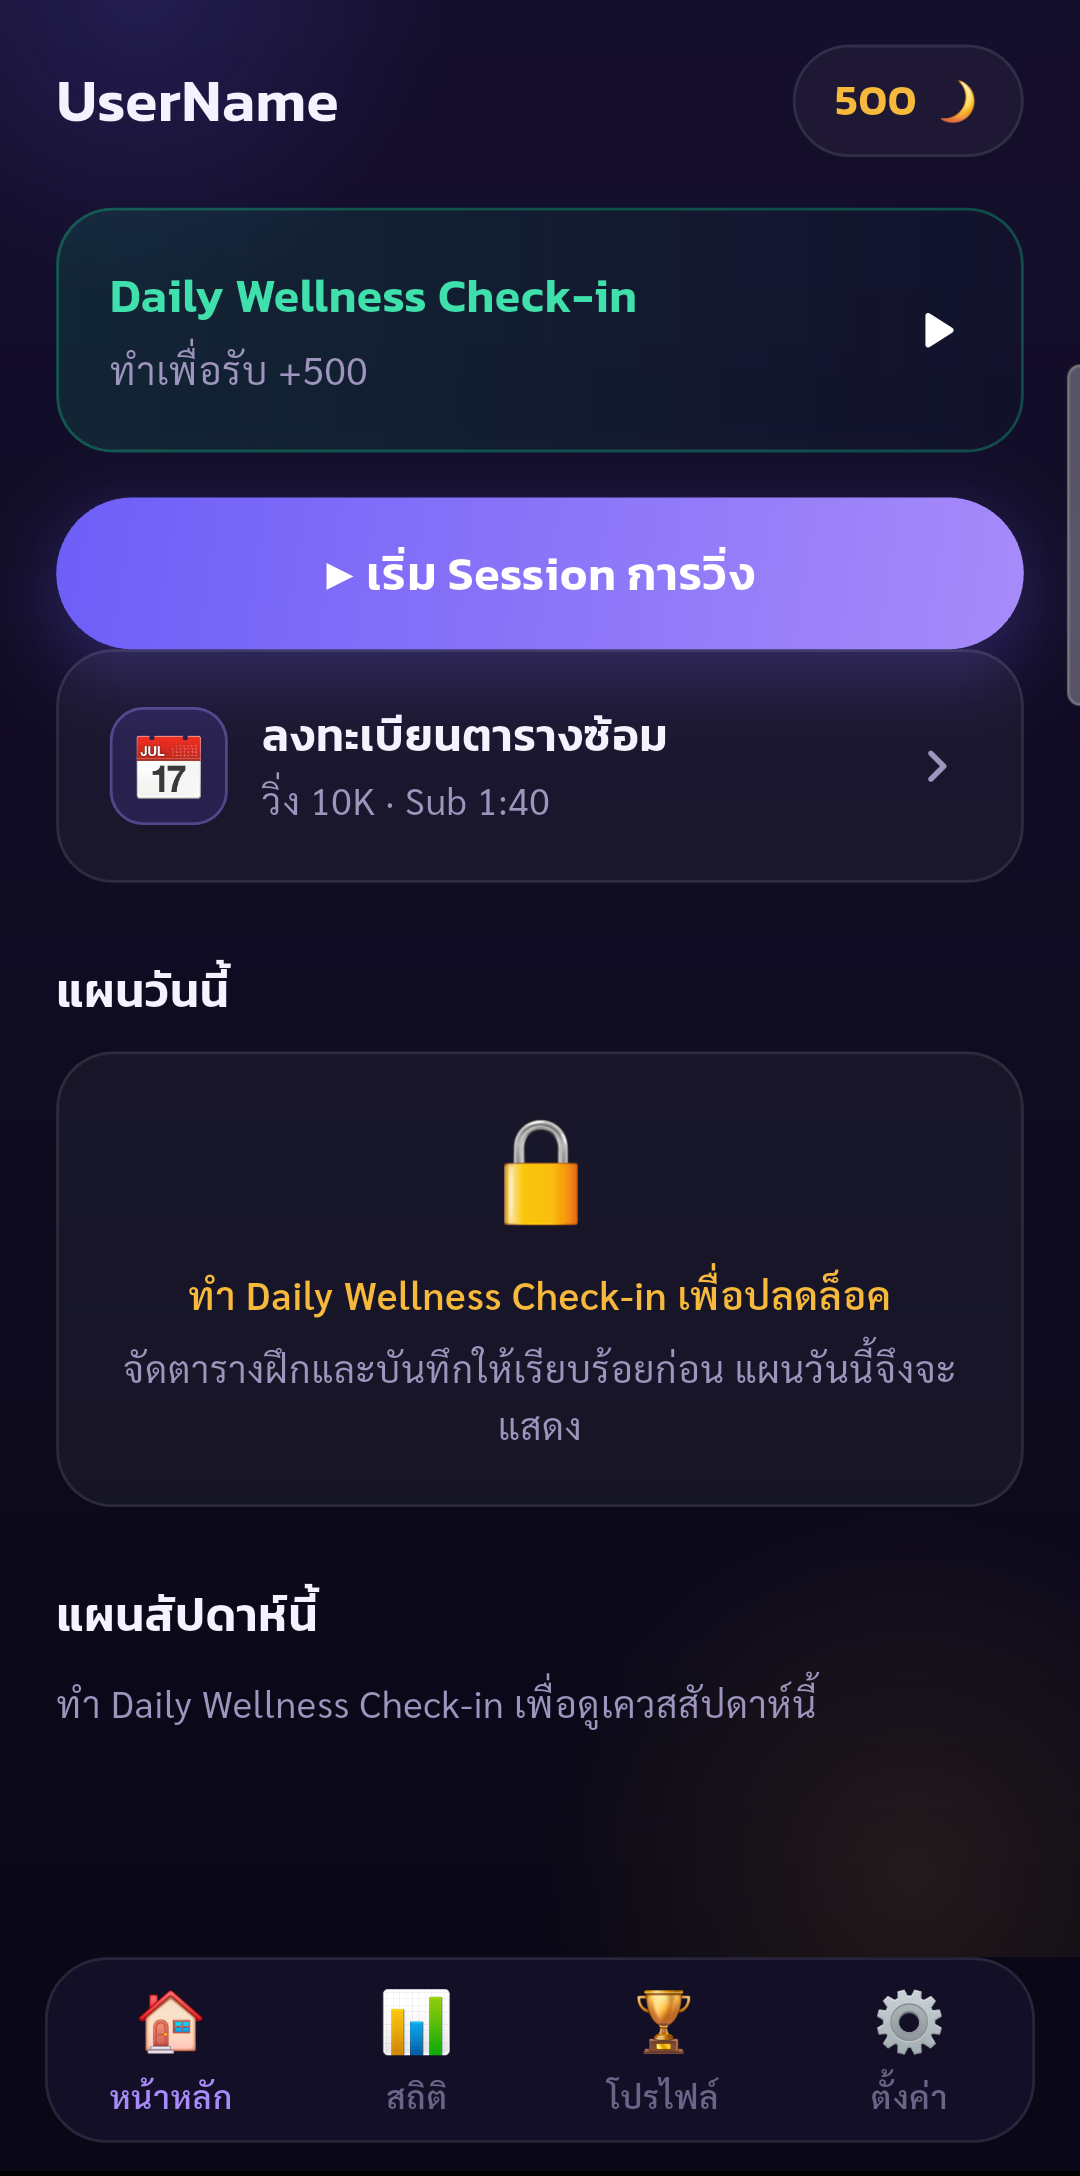
\includegraphics[width=\textwidth]{images/pegasus-home-locked.png}\caption{หน้าหลักก่อนปลดล็อก}\end{subfigure}\hfill
\begin{subfigure}[t]{0.31\textwidth}\centering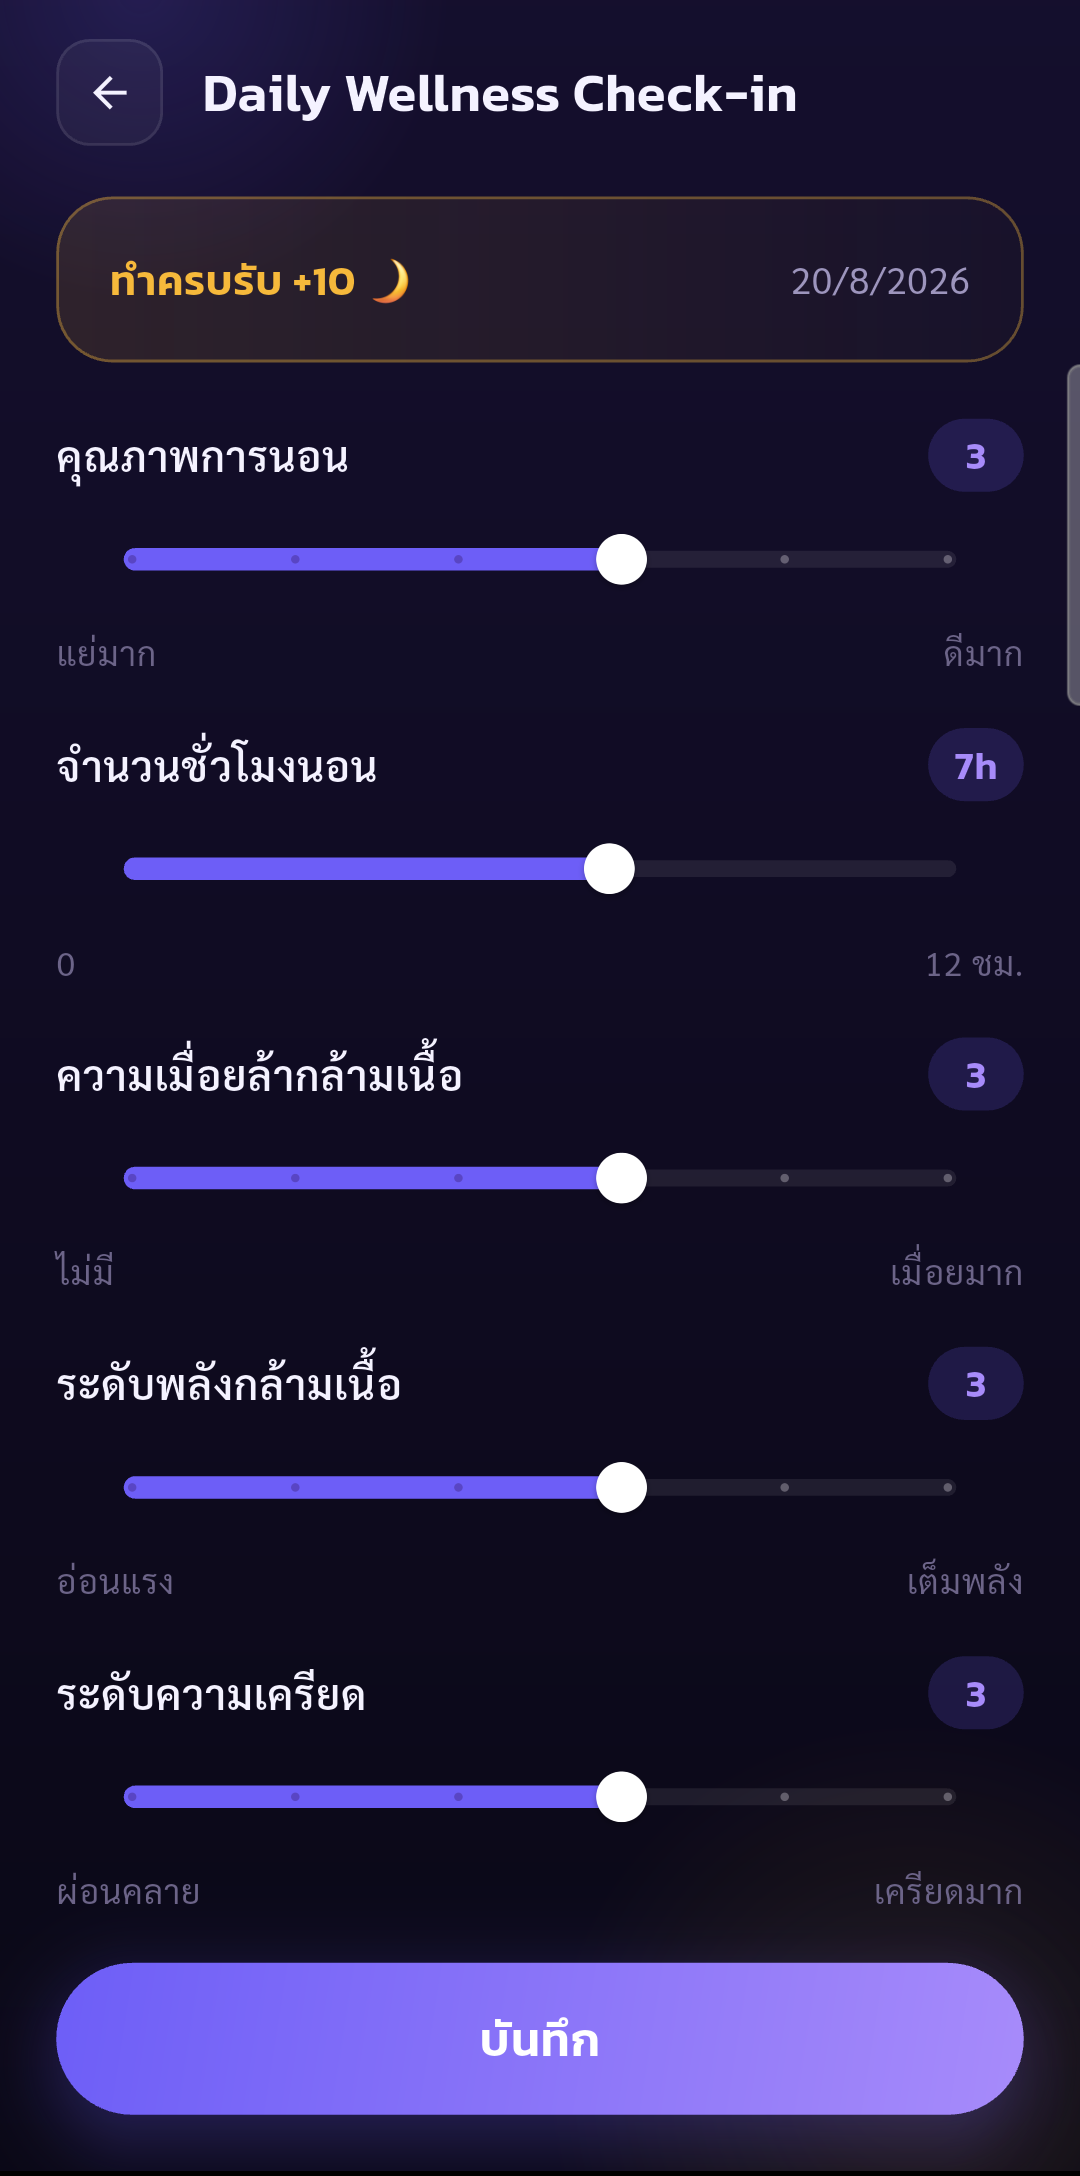
\includegraphics[width=\textwidth]{images/pegasus-daily-wellness-check-in.png}\caption{Daily Wellness Check-in}\end{subfigure}\hfill
\begin{subfigure}[t]{0.31\textwidth}\centering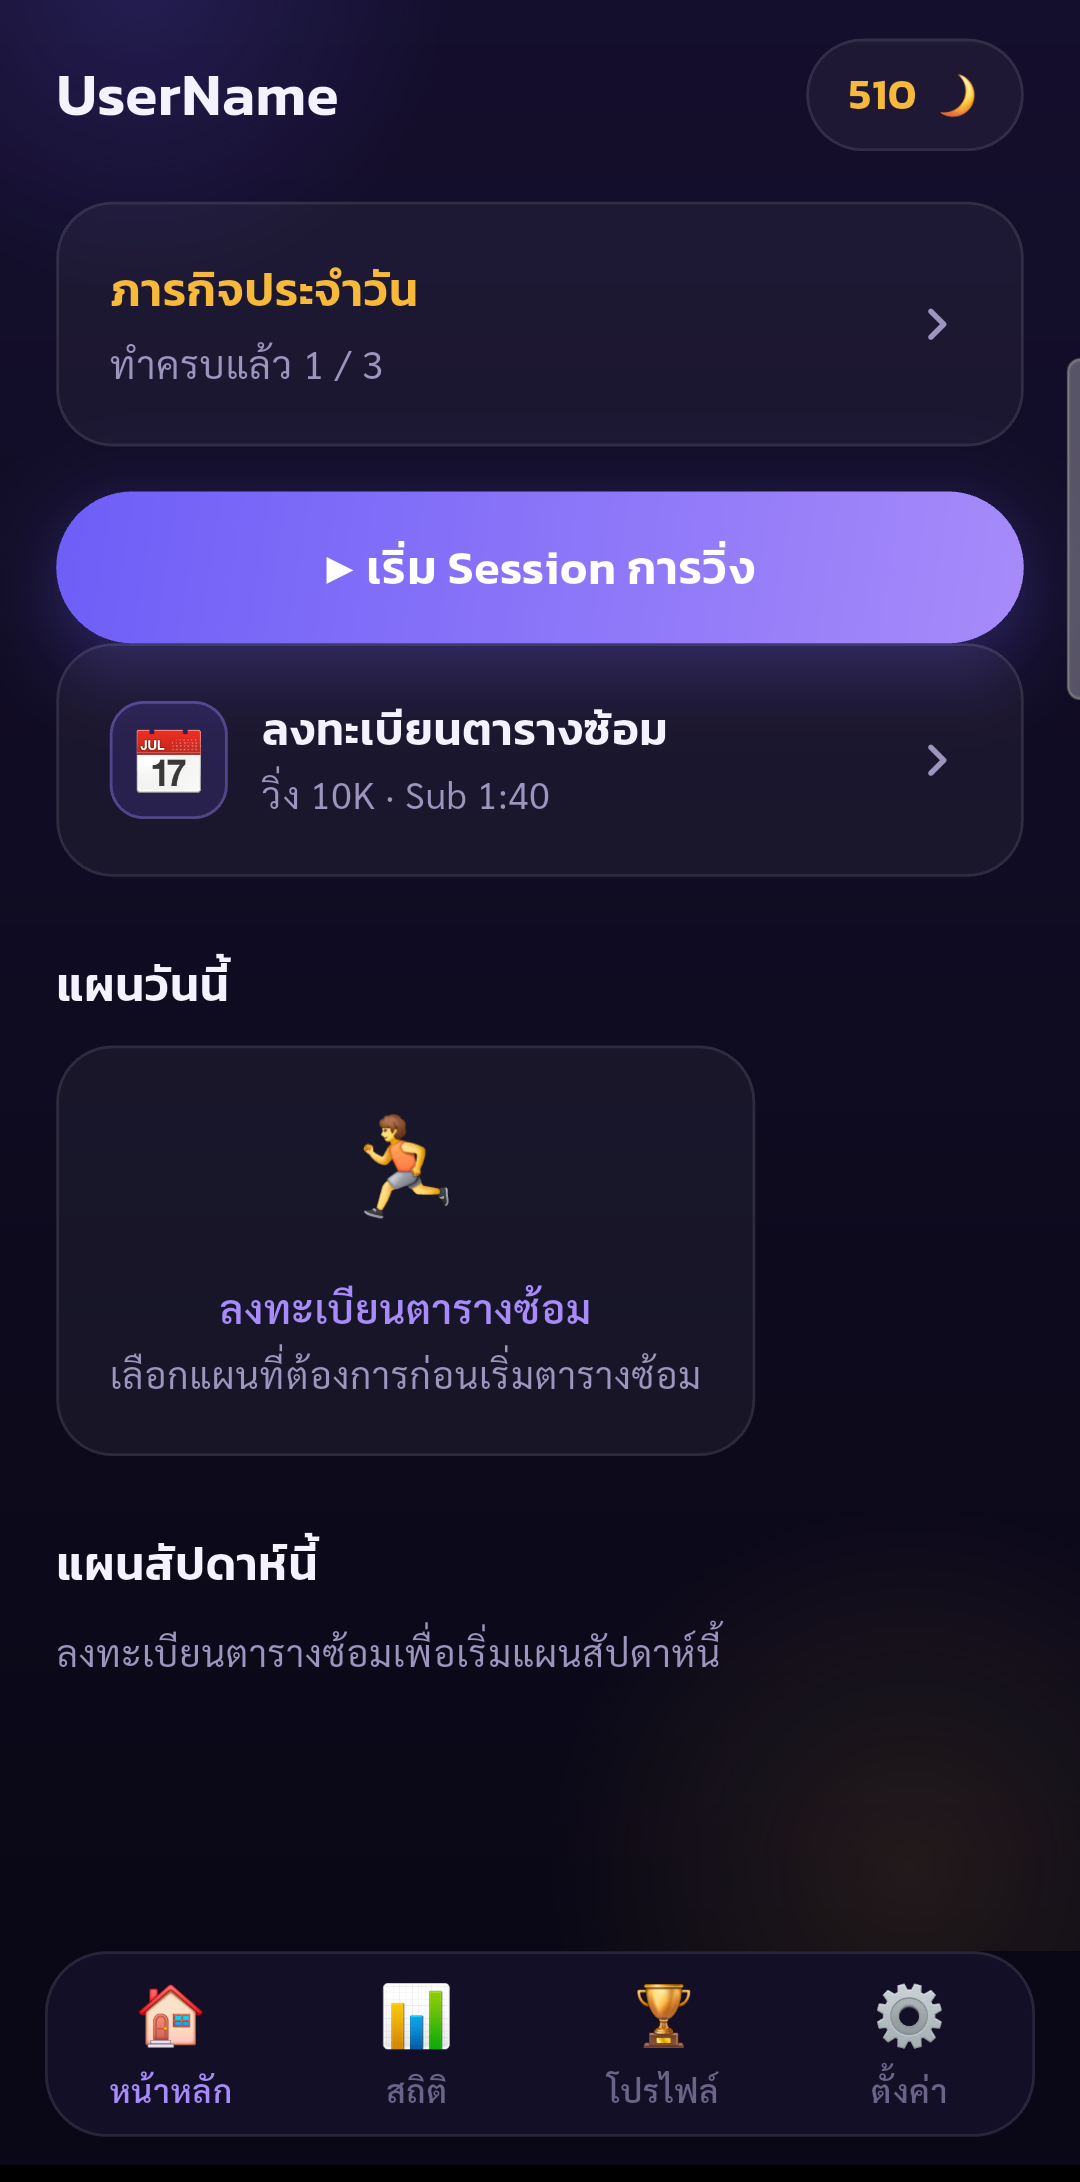
\includegraphics[width=\textwidth]{images/pegasus-home-training-required.png}\caption{หน้าหลักหลังการเช็กอิน}\end{subfigure}
\caption{หน้าหลักและการประเมินความพร้อมประจำวัน}\label{fig:app-home-wellness}
\end{figure}

\begin{figure}[H]\centering
\begin{subfigure}[t]{0.31\textwidth}\centering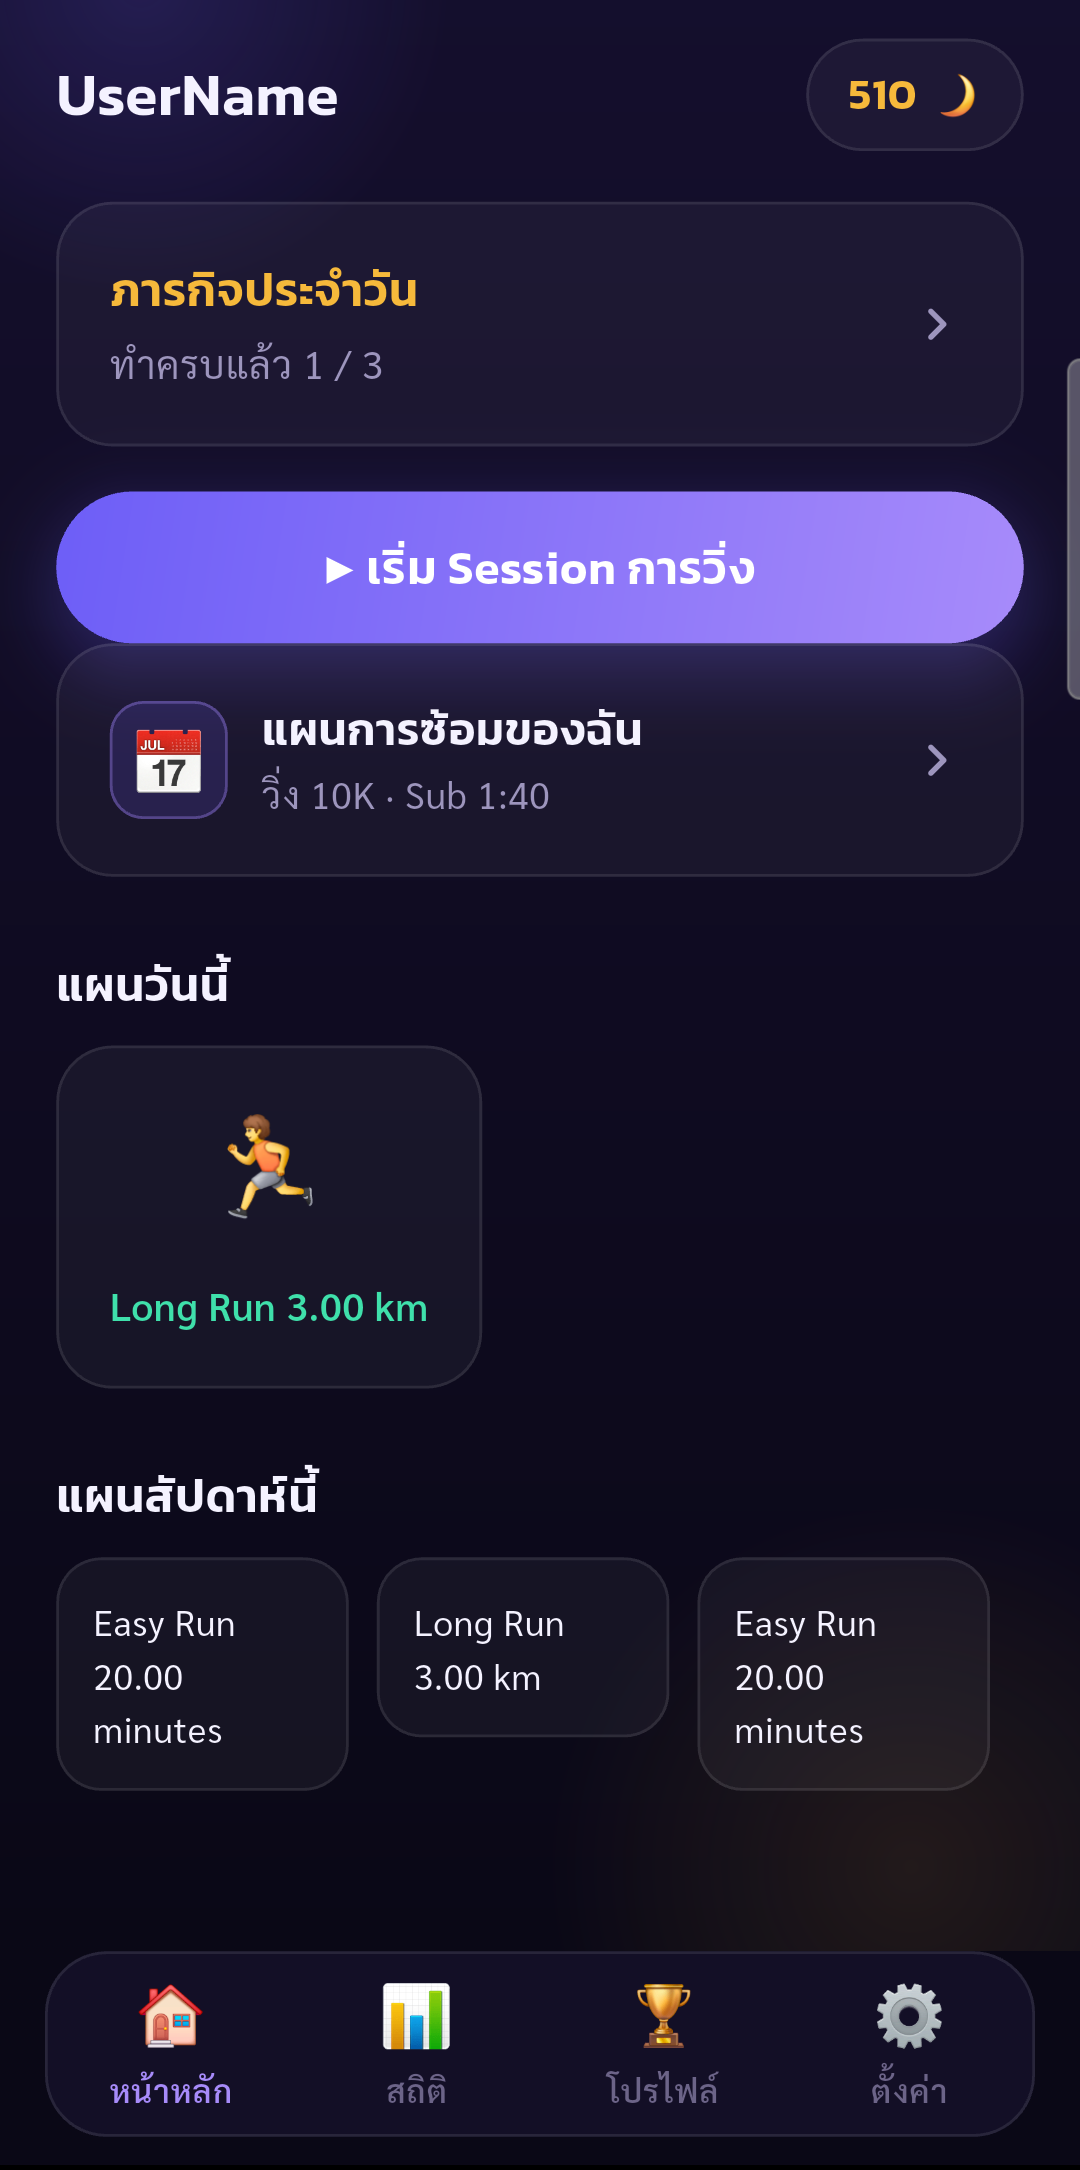
\includegraphics[width=\textwidth]{images/pegasus-home-training-scheduled.png}\caption{หน้าหลักพร้อมแผนฝึก}\end{subfigure}\hfill
\begin{subfigure}[t]{0.31\textwidth}\centering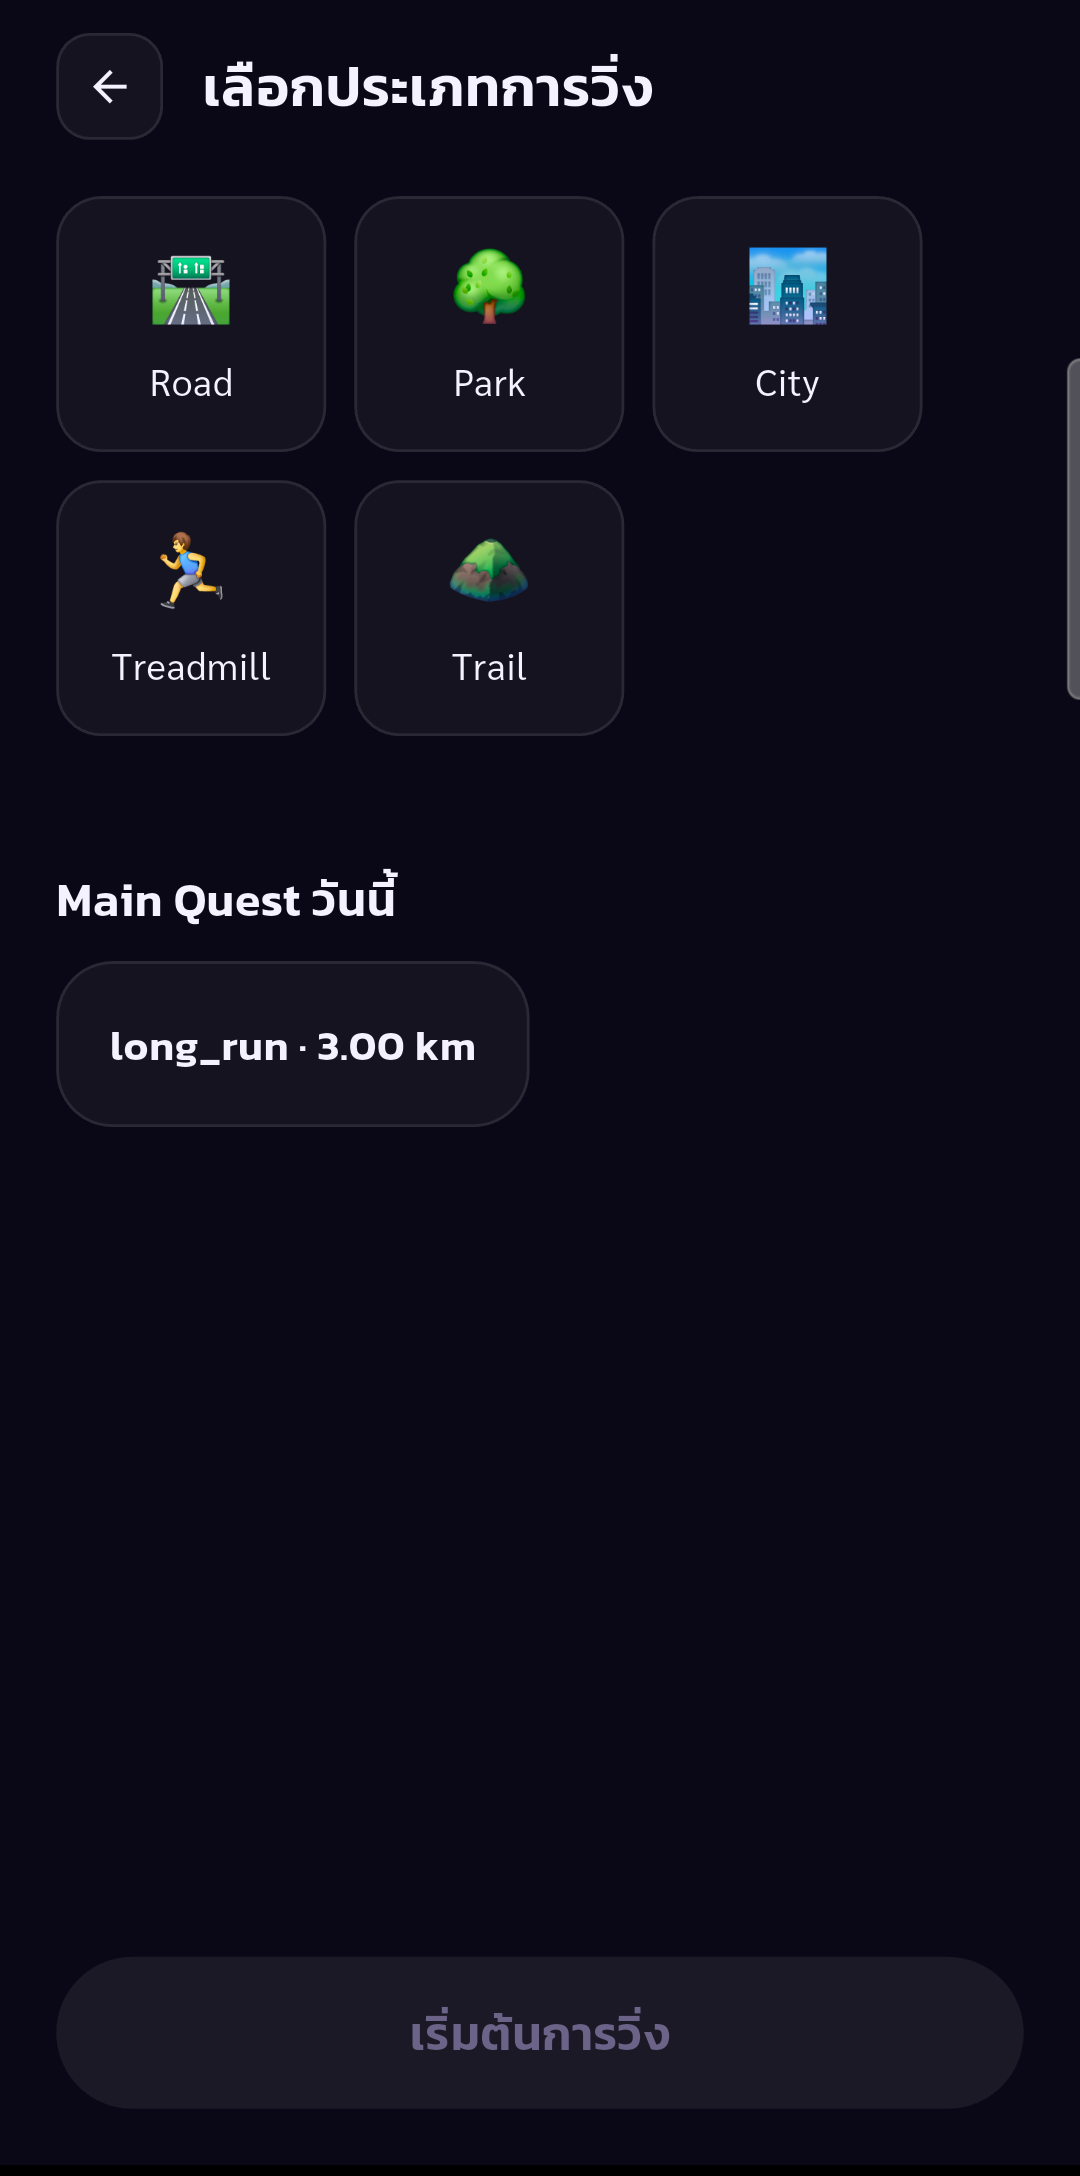
\includegraphics[width=\textwidth]{images/pegasus-run-session-type-selection.png}\caption{เลือกประเภทการวิ่ง}\end{subfigure}\hfill
\begin{subfigure}[t]{0.31\textwidth}\centering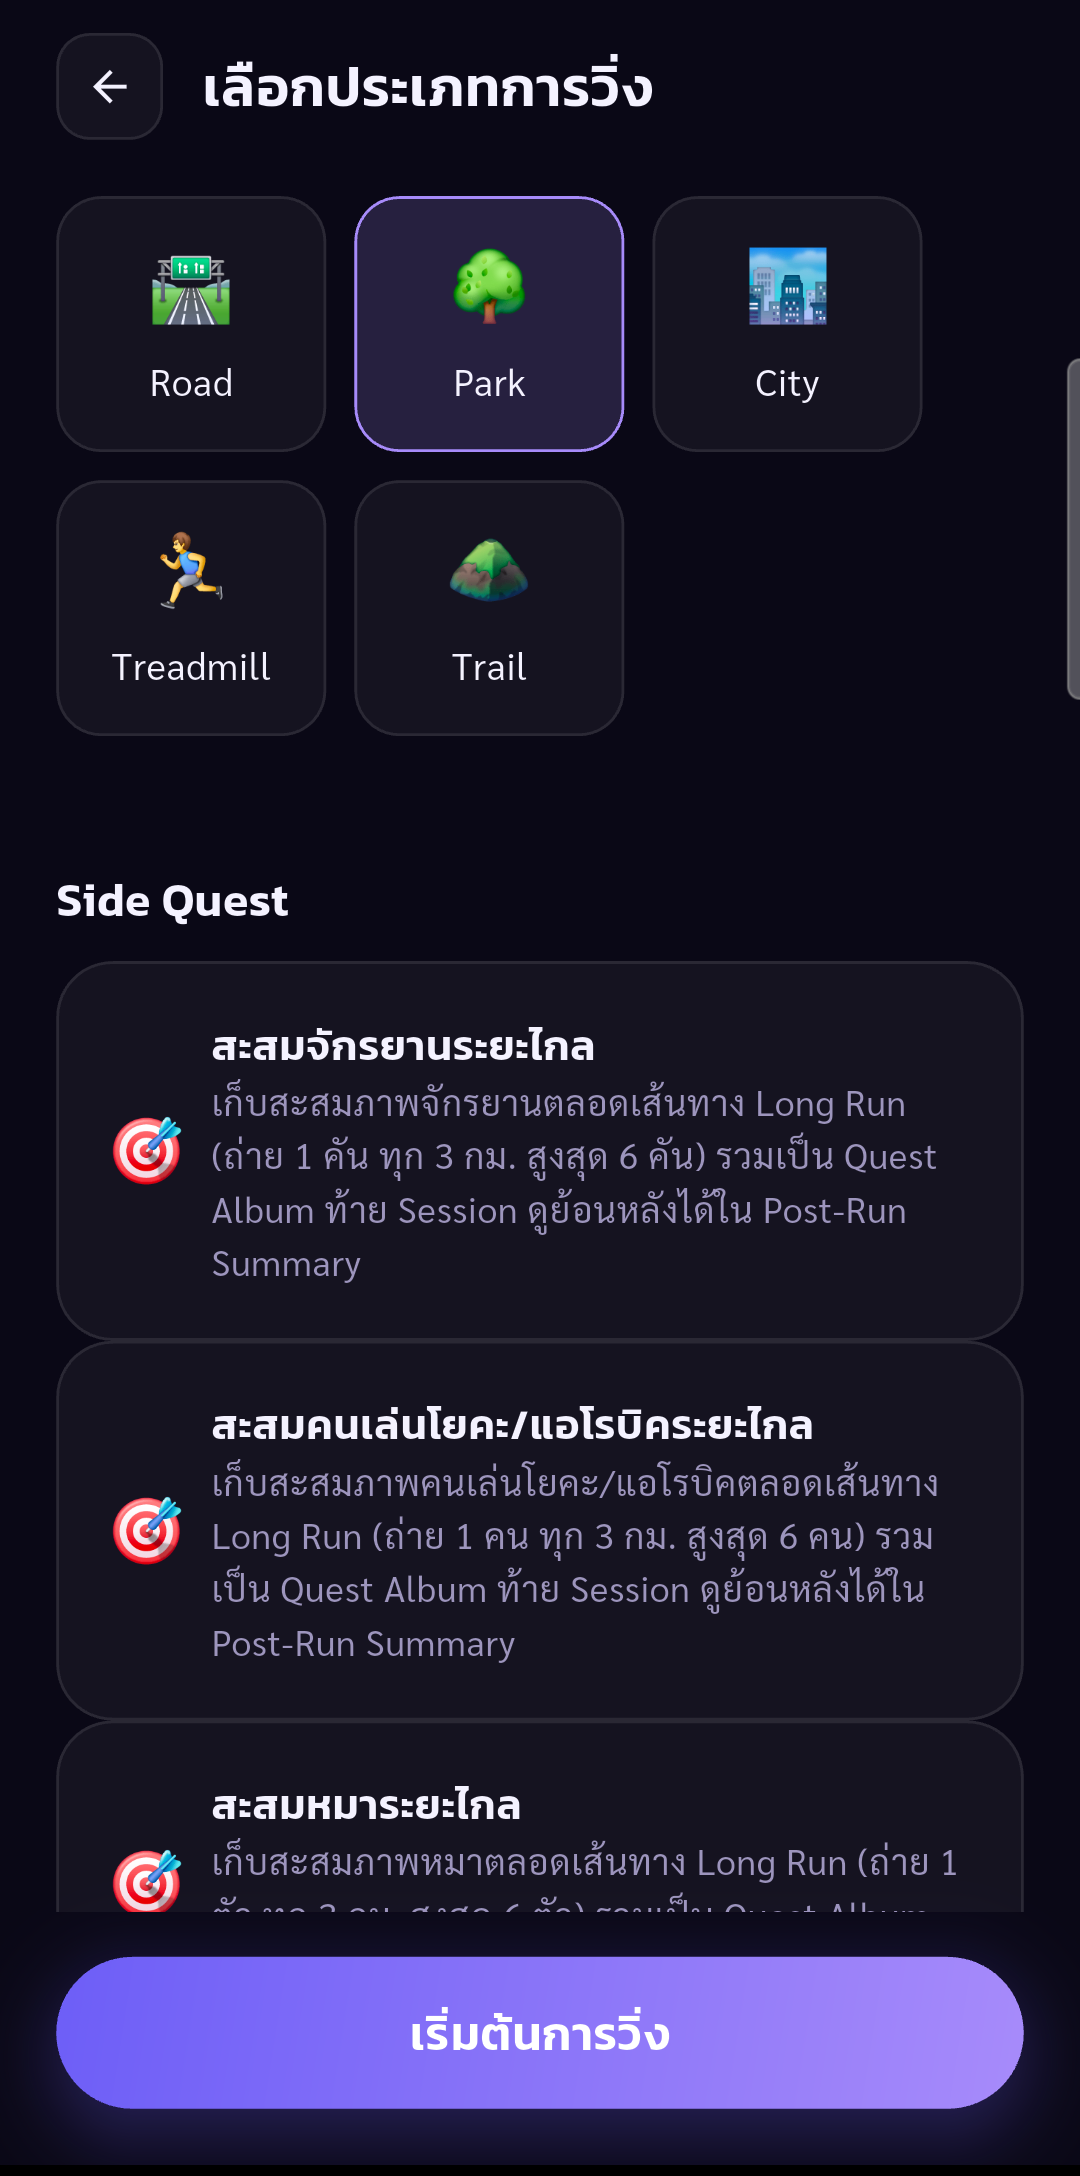
\includegraphics[width=\textwidth]{images/pegasus-run-session-quests.png}\caption{ภารกิจระหว่างการวิ่ง}\end{subfigure}
\caption{หน้าหลักและการเตรียมเริ่ม Session การวิ่ง}\label{fig:app-session-preparation}
\end{figure}

\subsection*{การวิ่งและผลลัพธ์หลังวิ่ง}

หน้าจอ Active Run Session แสดงเวลา ระยะทาง Pace ตำแหน่งบนแผนที่ และภารกิจที่กำลังดำเนินการ เมื่อจบการวิ่ง ระบบจะแสดงหน้าสรุปผลเพื่อให้ผู้ใช้ประเมิน RPE ระดับความเครียด และความรู้สึกหลังวิ่ง

\begin{figure}[H]\centering
\begin{subfigure}[t]{0.31\textwidth}\centering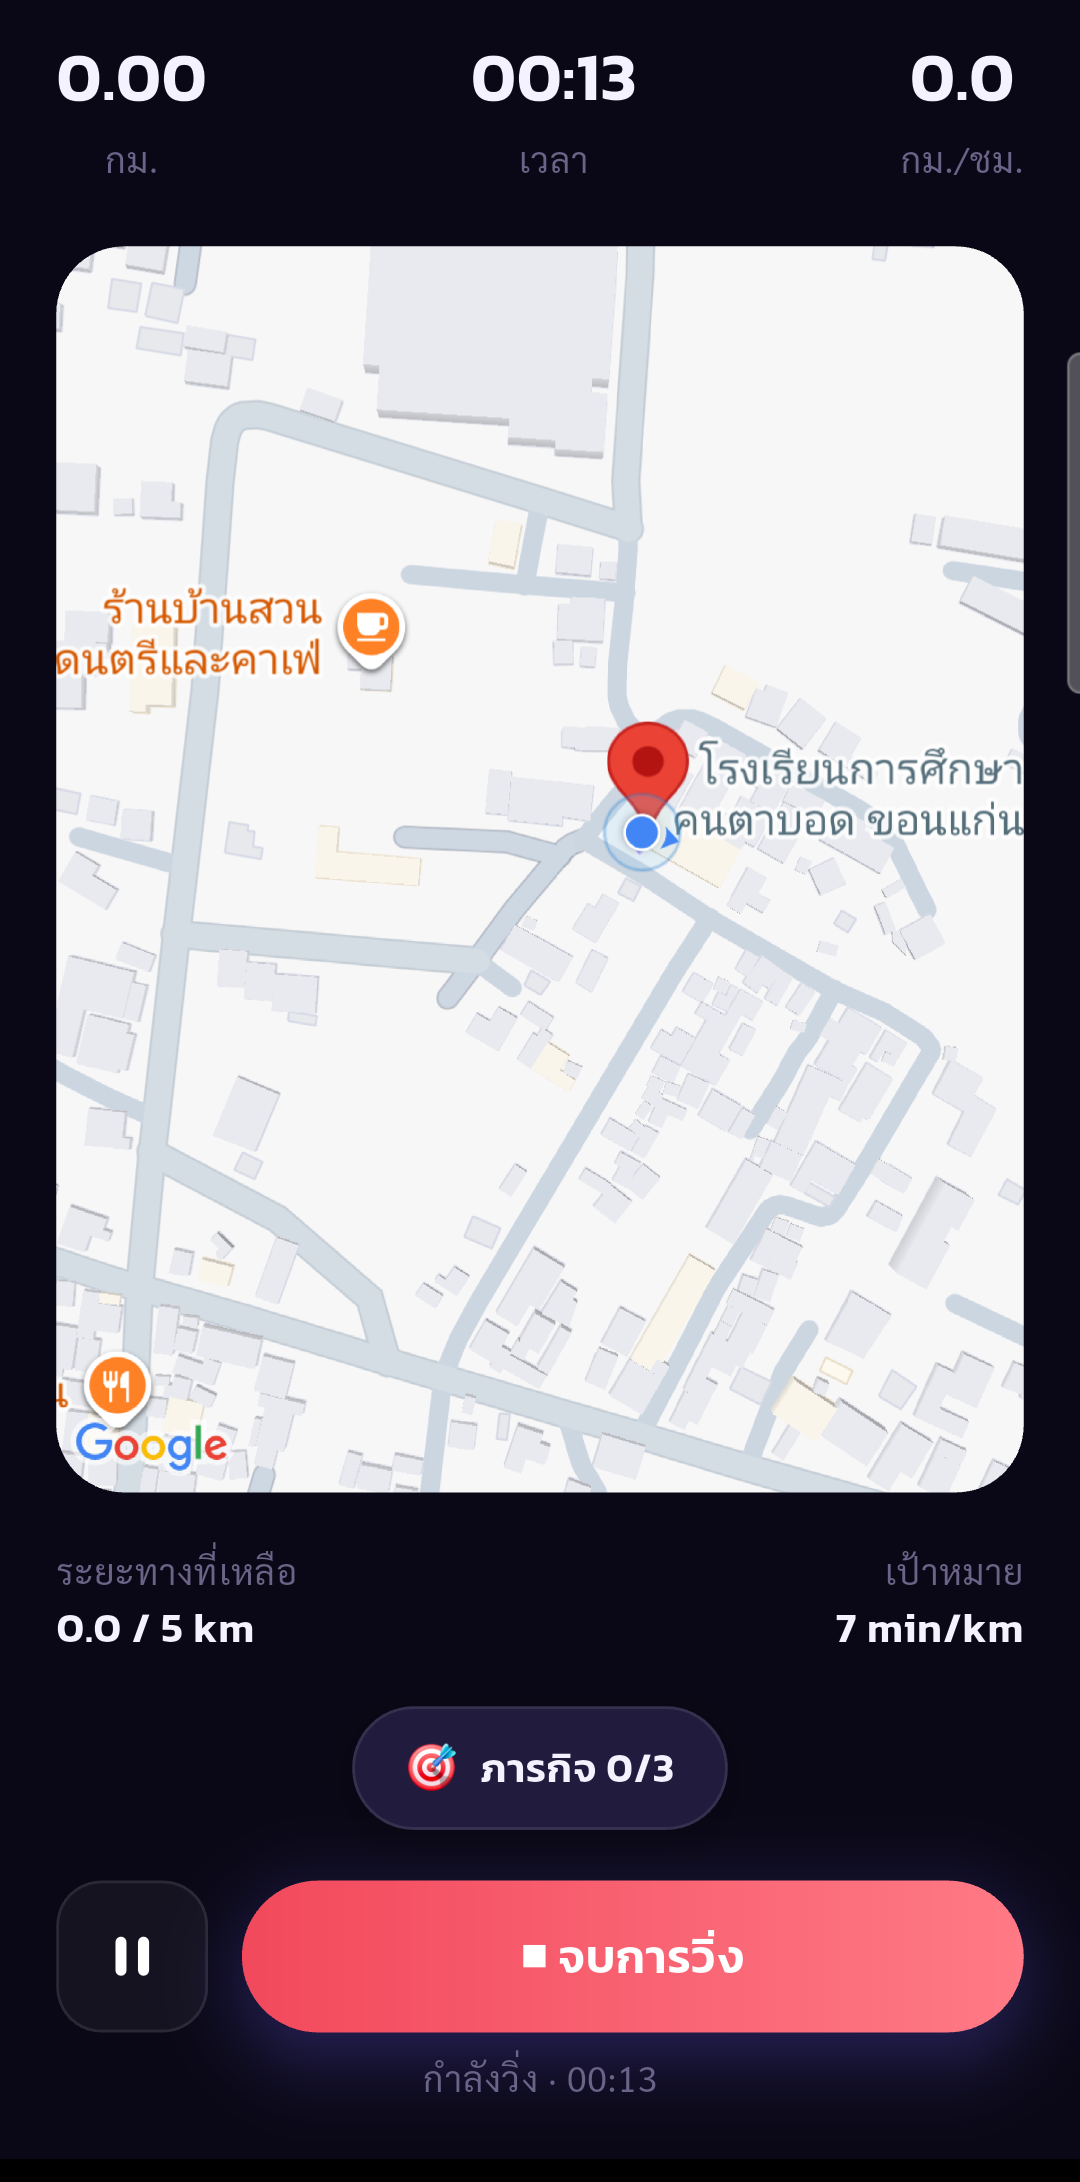
\includegraphics[width=\textwidth]{images/pegasus-active-run-session.png}\caption{กำลังวิ่ง}\end{subfigure}\hfill
\begin{subfigure}[t]{0.31\textwidth}\centering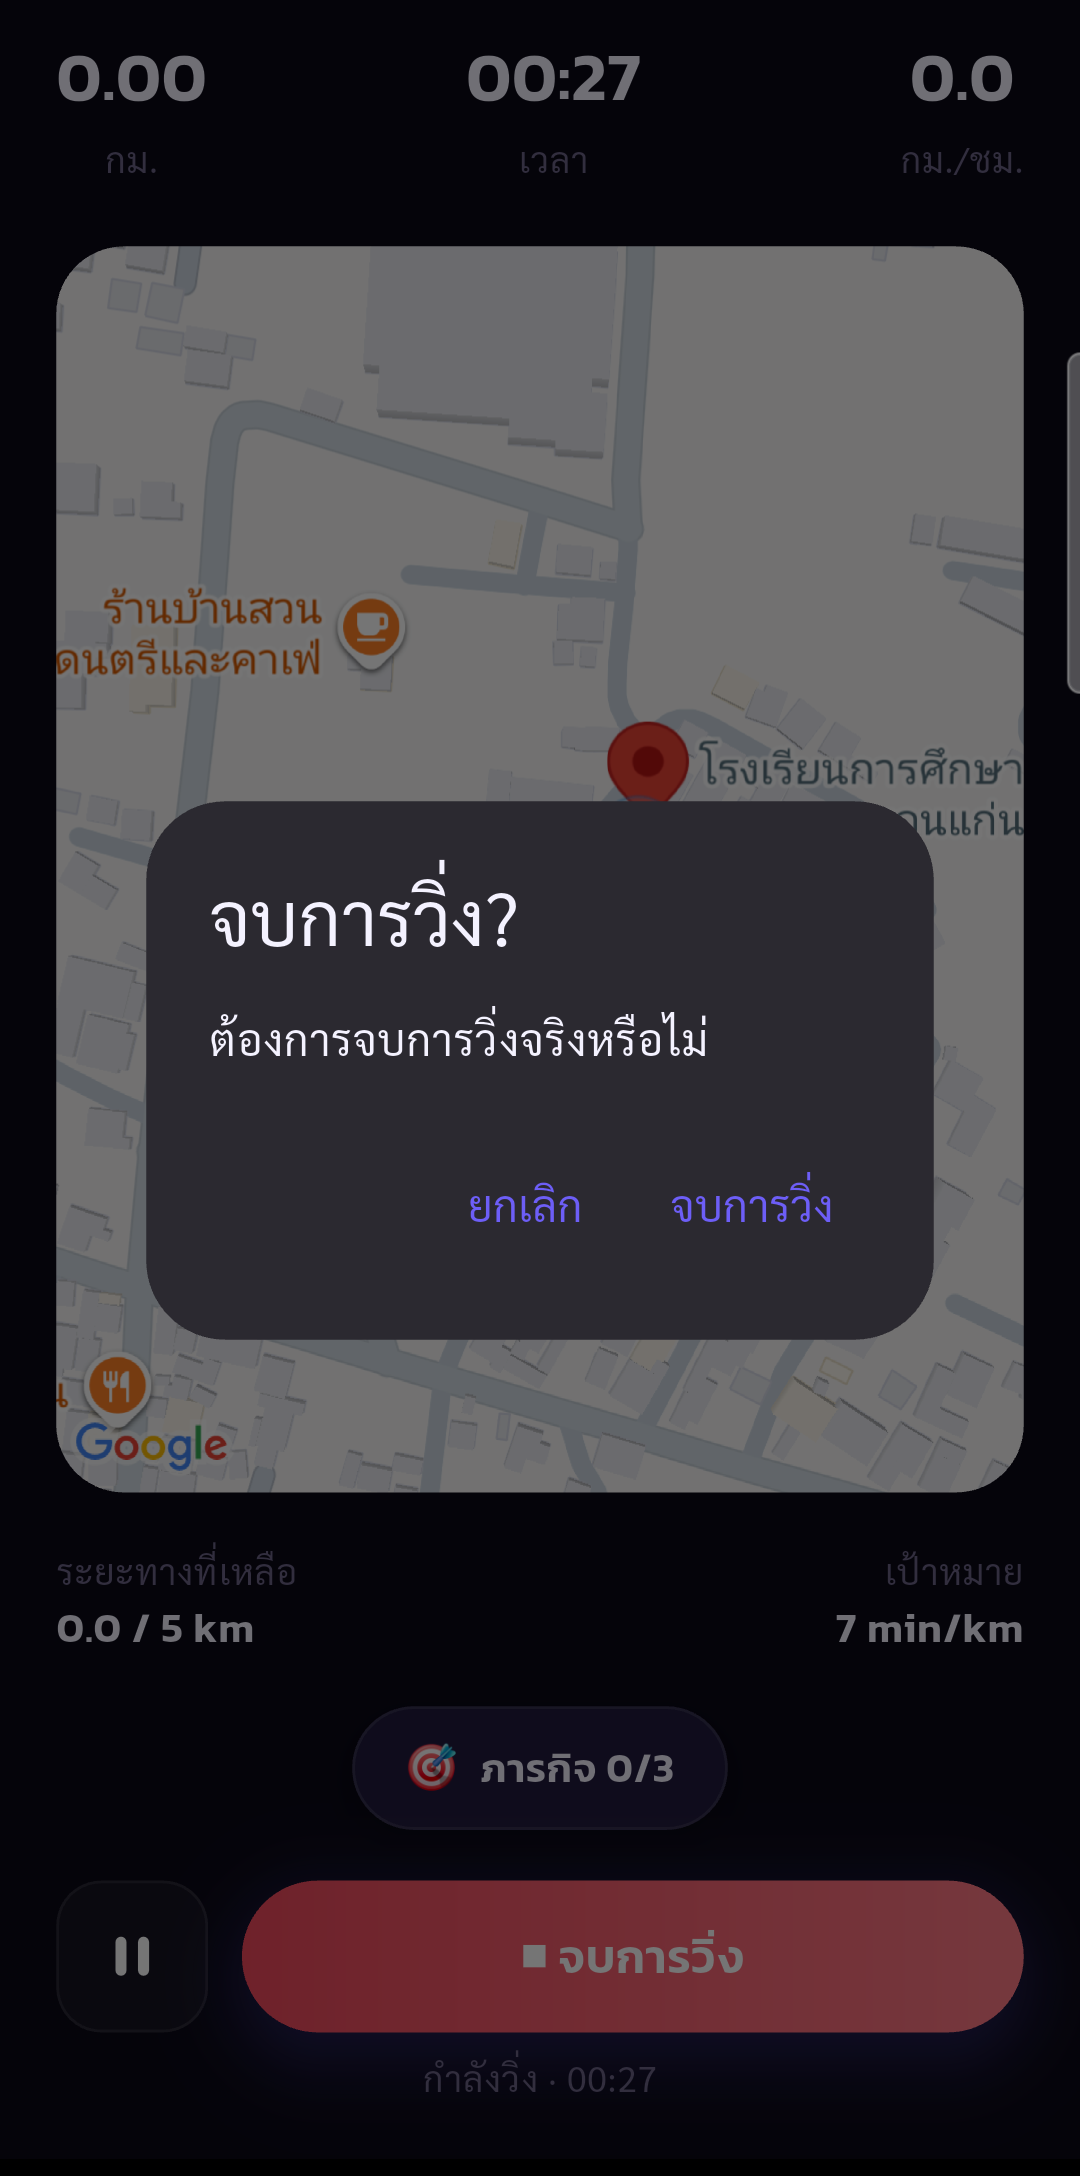
\includegraphics[width=\textwidth]{images/pegasus-end-run-confirmation.png}\caption{ยืนยันจบการวิ่ง}\end{subfigure}\hfill
\begin{subfigure}[t]{0.31\textwidth}\centering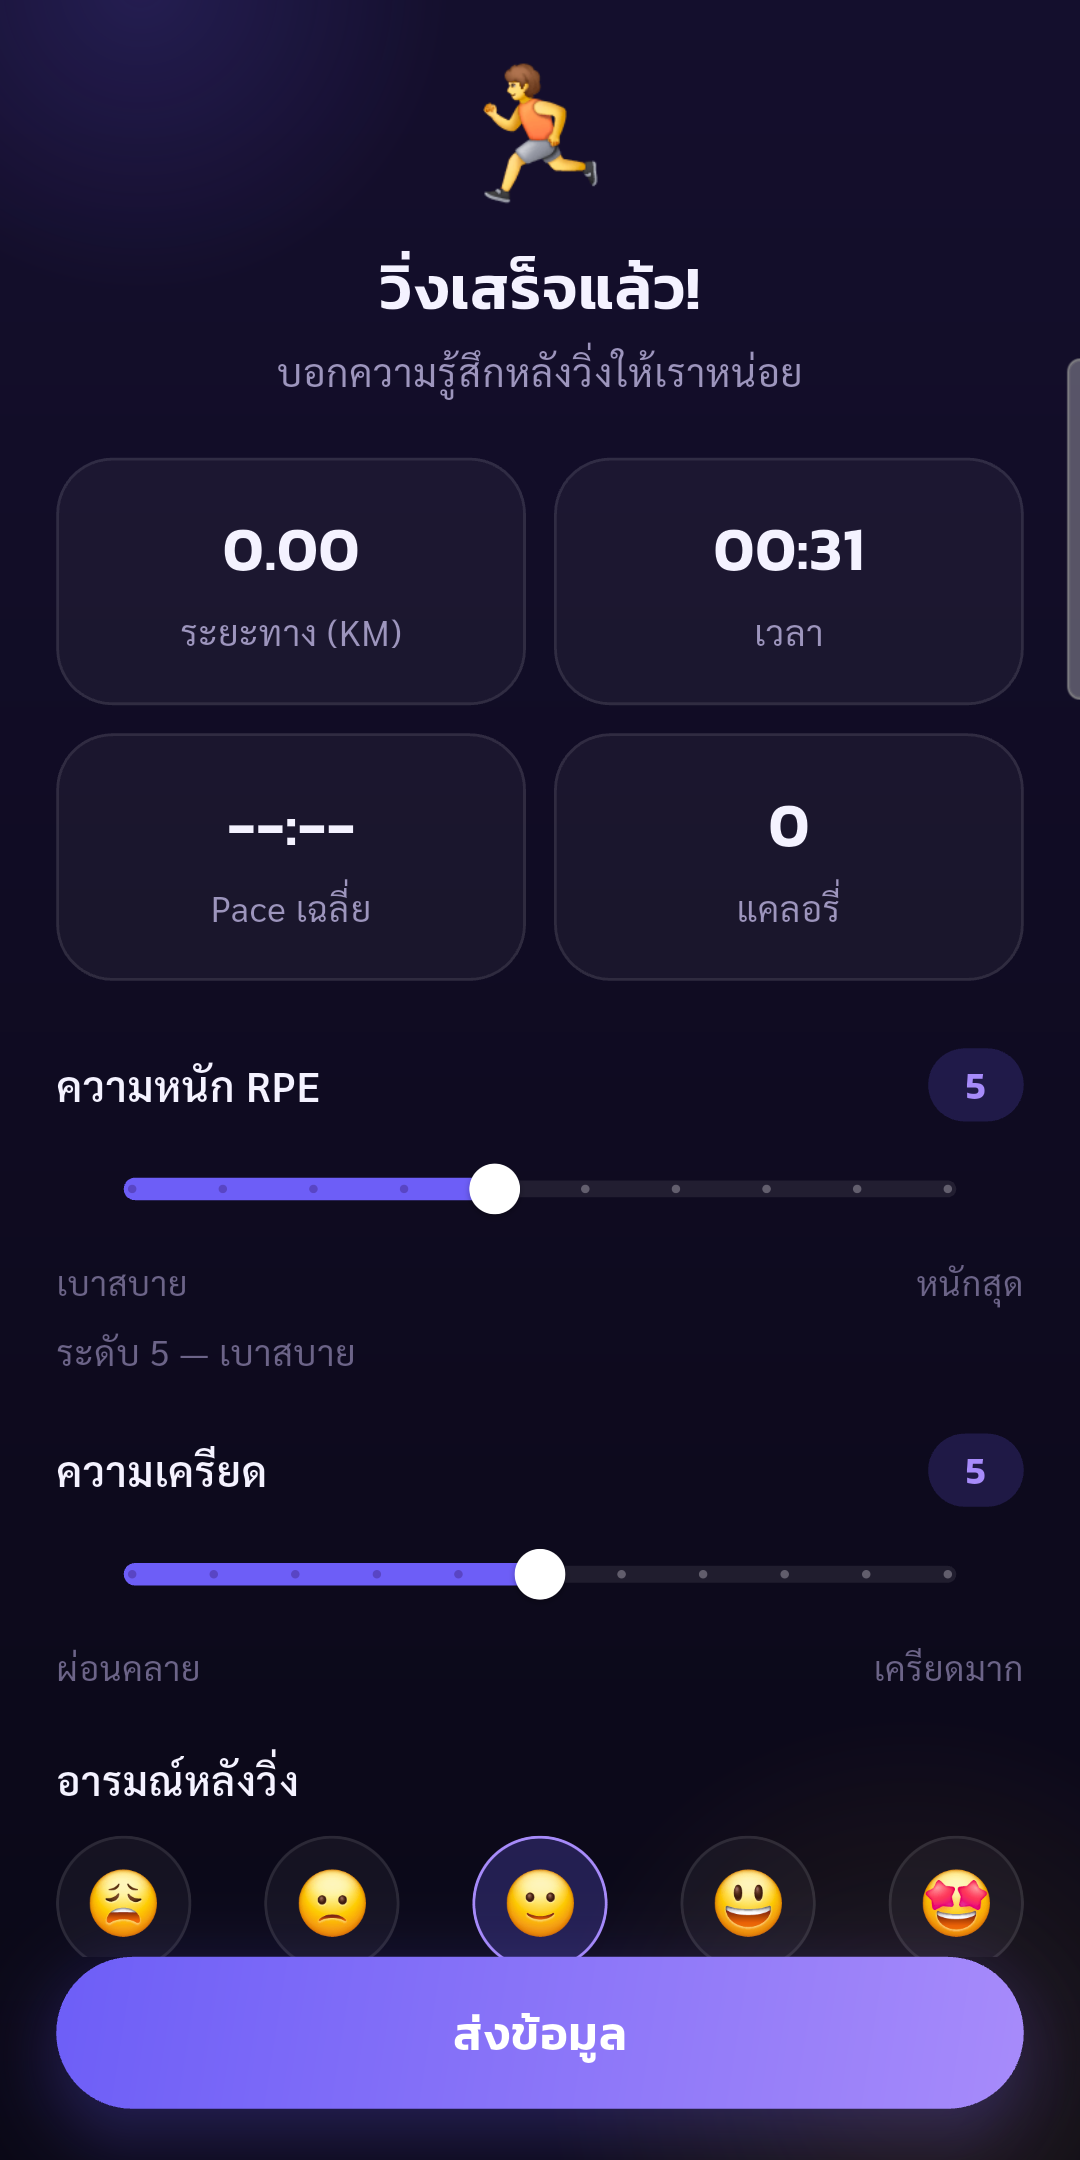
\includegraphics[width=\textwidth]{images/pegasus-post-run-feedback.png}\caption{สรุปผลและ Feedback}\end{subfigure}
\caption{หน้าจอการวิ่งและการประเมินหลังวิ่ง}\label{fig:app-running-result}
\end{figure}

\subsection*{ระบบรางวัลและ Gamification}

เมื่อผู้ใช้ทำกิจกรรมเสร็จ ระบบจะแสดงรางวัลเป็นเหรียญและคะแนนประสบการณ์ เพื่อสร้าง Feedback ทันทีและสนับสนุนให้ผู้ใช้กลับมาใช้งานอย่างต่อเนื่อง

\begin{figure}[H]\centering

\includegraphics[width=0.31\textwidth]{images/pegasus-run-rewards.png}
\caption{หน้าจอแสดงรางวัลหลังการวิ่ง}\label{fig:app-rewards}
\end{figure}

\section*{คู่มือการใช้งาน}

การใช้งานระบบเริ่มจากการสมัครสมาชิกหรือเข้าสู่ระบบ จากนั้นกรอกข้อมูลพื้นฐานและข้อมูลสุขภาพ เลือกเป้าหมายและแผนการฝึก ทำ Daily Wellness Check-in ก่อนเริ่มวิ่ง บันทึกผลการวิ่ง และตรวจสอบผลลัพธ์รวมถึงรางวัลหลังวิ่ง

% =============================
% ภาคผนวก ข (ตัวอย่าง — uncomment ถ้าต้องการ)
% =============================
% \appendiceschapter{รายละเอียดเพิ่มเติม}
% \section*{หัวข้อ}
% เนื้อหาภาคผนวก ข


% ==========================================
% ประวัติผู้เขียน
% ==========================================
\begin{biography}
% ประวัติผู้เขียน
% หมายเหตุ: ไม่เกิน 1 หน้ากระดาษ
%
% *** ลบข้อความตัวอย่างด้านล่าง แล้วเขียนประวัติของตนเอง ***

\section*{นักศึกษาคนที่ 1}

นาย พีรัชชัย สืบสิงห์ เกิดเมื่อวันที่ 12 พฤษภาคม พ.ศ. 2548 
สำเร็จการศึกษาระดับมัธยมศึกษาตอนปลาย จากโรงเรียน แก่นนครวิทยาลัย 2 เมื่อปีการศึกษา 2565
ปัจจุบันกำลังศึกษาระดับปริญญาตรี หลักสูตรวิทยาศาสตรบัณฑิต
สาขาวิชาวิทยาการคอมพิวเตอร์ วิทยาลัยการคอมพิวเตอร์ มหาวิทยาลัยขอนแก่น


\section*{นักศึกษาคนที่ 2}

นายเบญจพล บุบผามาลา เกิดเมื่อวันที่ 3 กรกฏาคม พ.ศ. 2547
สำเร็จการศึกษาระดับมัธยมศึกษาตอนปลาย จากโรงเรียนเบญจมราชูทิศ จังหวัดจันทบุรี เมื่อปีการศึกษา 2565
ปัจจุบันกำลังศึกษาระดับปริญญาตรี หลักสูตรวิทยาศาสตรบัณฑิต
สาขาวิชาวิทยาการคอมพิวเตอร์ วิทยาลัยการคอมพิวเตอร์ มหาวิทยาลัยขอนแก่น
\end{biography}

\end{document}
